\section{Estimation and Results} \label{sec:estim_res}
We investigate the heterogeneity of the Marginal Propensity to Consume by estimating the following partially linear model
\begin{align}
    \Delta C_{it+1}&=\theta(X_{it})R_{it+1}+g(X_{it}, W_{it})+\epsilon_{it} \label{eq:plm_C1}\\
    R_{it+1}&=h(X_{it}, W_{it})+u_{it} \label{eq:plm_C2}
\end{align}
where our outcome of interest is the change in consumption between two quarters, $\Delta C_{it+1}$ and our treatment is the rebate amount, $R_{it}$, household $i$ receives. The choice of confounders $X_{it}$ and $W_{it}$ depends on the specification we estimate, as does which variables we consider to be part of $X_{it}$ and thus have an effect on the treatment effect. Which variables are included in each specification is listed in Table \ref{tab:specs}. We follow Parker et al. by including monthly dummies in $W_{it}$ to account for seasonality and to capture any unobserved effects that might appear in periods in which households learn about the upcoming rebate. By canceling these effects stemming from the anticipation of the treatment, our estimate represents the effect of actually receiving the rebate. \\ 
In total, we distinguish between three different layers in our estimations: we investigate different outcomes $\Delta C_{it+1}$ by using the rich information on expenditure categories included in the CEX. With the term 'specification' we distinguish between the different sets of confounders $X_{it}$ and $W_{it}$ we use. Lastly, we estimate each outcome-specification pair twice: once using the linear and once using the causal forest second stage. Since our estimation procedure predicts MPCs and we can retrieve standard errors for each household, we can run hypothesis tests on whether their response to the tax rebate is statistically significant.
\begin{table}[t]
\begin{threeparttable}
\begin{tabular}{l c c}
\toprule 
Specification & $X_{it}$ & $W_{it}$ \\ 
1 & Age, change in family size & \\
2 & & \\ 
3 & & \\  
\end{tabular}
\end{threeparttable}
\caption{Specifications}
\label{tab:specs}
\end{table}
However, one drawback in our specification including liquidity, salary, and income - which we also refer to as the \textit{financial status} - is the already mentioned lack of detailed documentation of household characteristics in the CEX. Our sample size shrinks because they are not consistently documented for each interviewed household. This sample reduction can induce a sample selection bias because it is possible that households answering questions on their liquidity are systematically different from households that do not provide such information. We have to keep this drawback in mind although the DML framework achieves fast convergence rates even in cases in which the first stage predictions do not converge rapidly.

\subsection{Identifying the Income Shock} \label{subsec:identification}
Since we use the same event and data source to estimate the MPC, our baseline identification approach is similar to \cite{parkeretal_2013}. The key factor is the design of the stimulus rollout, which we exploit to identify the income shock. The tax stimulus was paid out to households over several weeks as administrative and technological restrictions made it impossible to pay out all rebates at once. Instead, the date of rebate receipt depended on the last two digits of tax filers' social security number. These digits are randomly distributed, and therefore the timing of the treatment is random, rendering it exogenous from any household characteristics. Therefore, we observe rebate receipts at different points in time, which allows us to use all other households that received their rebate in a different quarter as the control group. \\
Parker et al. identify a potential source of bias in this identification approach. They argue that using the actual amount of tax rebate received can lead to an omitted variable bias. This concern arises because of how households' stimulus payments are determined. Remember that the tax rebate directly depends on the number of children, which certainly affects the absolute level of households' expenditures, as each dependent child adds 300 USD to the stimulus received. However, this is not a problem because we can control for the number of children in each specification. \\
The stimulus excluding the child bonuses equals the household's net income tax liability (NTL; in the following, also referred to as the net tax liability) as long as it is within the exogenously defined boundaries we discussed in Section \ref{subsec:stimulus_desc}. Parker et al. argue that the NTL might also drive changes in consumption, rendering the treatment endogenous. Their solution is to instrument the amount received with a dummy variable that only signals whether the stimulus was received or not in the given quarter. While their results and the authors themselves suggest that this is not much of a concern, we decisively disagree with their identification approach in general. \\
Parker et al. do not control for any variable related to households income or salary. These variables are without a doubt directly connected to our treatment because the NTL - i.e., how much a household owes in income taxes - is a function of the household's income. Excluding these variables leads to omitted variable bias causing inconsistent estimates. However, other than through the channel of income, we deem it highly unlikely that the net tax liability itself is driving changes in consumption. It might be possible that in other years the NTL plays a role for households' income as it can be perceived as an anticipated income - or liquidity - shock.\footnote{Households usually should know that they will have to pay this or receive this because of past experience and because the NTL also depends on how much income tax was already paid during the previous year.} However, in 2008, the NTL affected households via their tax rebate, i.e., it does not affect the consumption change through other channels than what is captured by the tax rebate. Therefore, we argue in favor of using the actual rebate amount since it has two advantages: for one, we have an additional source of variation, and second, it allows us to estimate the continuous treatment effect and interpret it as the actual MPC. Moreover, this is in line with \cite{misrasurico_2014} whose results also suggest that the endogeneity of the NTL is not a concern.

\subsection{Main Results} \label{subsec:main_res}
We analyze our results in several steps and begin by looking at the empirical distribution of the estimated MPCs. Figures \ref{fig:dist_tot} to \ref{fig:dist_fd} shows the distribution of MPCs for the four main expenditure categories considered by Parker et al.: Total (Tot), Non-Durables (ND), Strictly Non-Durables (SND) as defined by \cite{lusardi_1996}, and Food (FD) expenditures. These categories are decreasing in their level of aggregation, e.g., SND includes expenditures on food. A detailed list of all sub-components of each of these categories is listed in Appendix \ref{app:c_cats}. Here, we only want to highlight that the difference between SND and ND consumption categories are so-called 'semi-durables,' such as health expenditures, which are not included in the SND category. 
\begin{table}[t]
    \label{tab:sig_shares}
    \centering
    \begin{threeparttable}
        \begin{tabular}{l @{\extracolsep{\fill}} cc}
            \toprule
            & Linear Estimator & Causal Forest Estimator \\
            \midrule
            Specification 1 & 0.615 & 0.128 \\
            \vspace{2pt}
            Specification 2 & 0.459 & 0.179 \\
            \vspace{2pt}
            Specification 3 & 0.0 & 0.102 \\
            \bottomrule
        \end{tabular}
    \begin{tablenotes} 
        \footnotesize
        \item The table reports shares of individuals that have a statistically significant MPC using the respective estimator. Significance at $p\leq0.1$. Outcome: change in non-durable expenditures.
    \end{tablenotes}
    \end{threeparttable}
\caption{Shares of significant MPCs - Non-Durable Expenditures}
\end{table}
\noindent A single plot of the empirical distribution as shown below is retrieved as follows. We slice the range between the minimum and maximum of the point estimates into 20 equidistant bins and calculate the share of estimated MPCs that fall into each bin. The x-axis signals the borders of the different bins, and the y-axis shows the respective frequency. The blue part of a bar signals the total frequency of this bin. To illustrate how many of these estimates are actually rejecting the null of a zero MPC, we calculate the share of point estimates that reject the null at the 10\% level within each bin. This is depicted by the red part of the frequency bars. I.e., a completely red bar implies that all observations within this bin are statistically significant, whereas a bar that is only red up to half of its height signals that this only holds for half of the point estimates within this bin. The vertical dashed line marks the average CATE - the average treatment effect across all households - as a benchmark. Note that the ATE is only significant for total expenditures but as soon as we control for the \textit{financial status} this significance vanishes.
\begin{figure}[t]
    \centering
%    \mbox{}\hfill
    \begin{subfigure}{0.33\linewidth}
        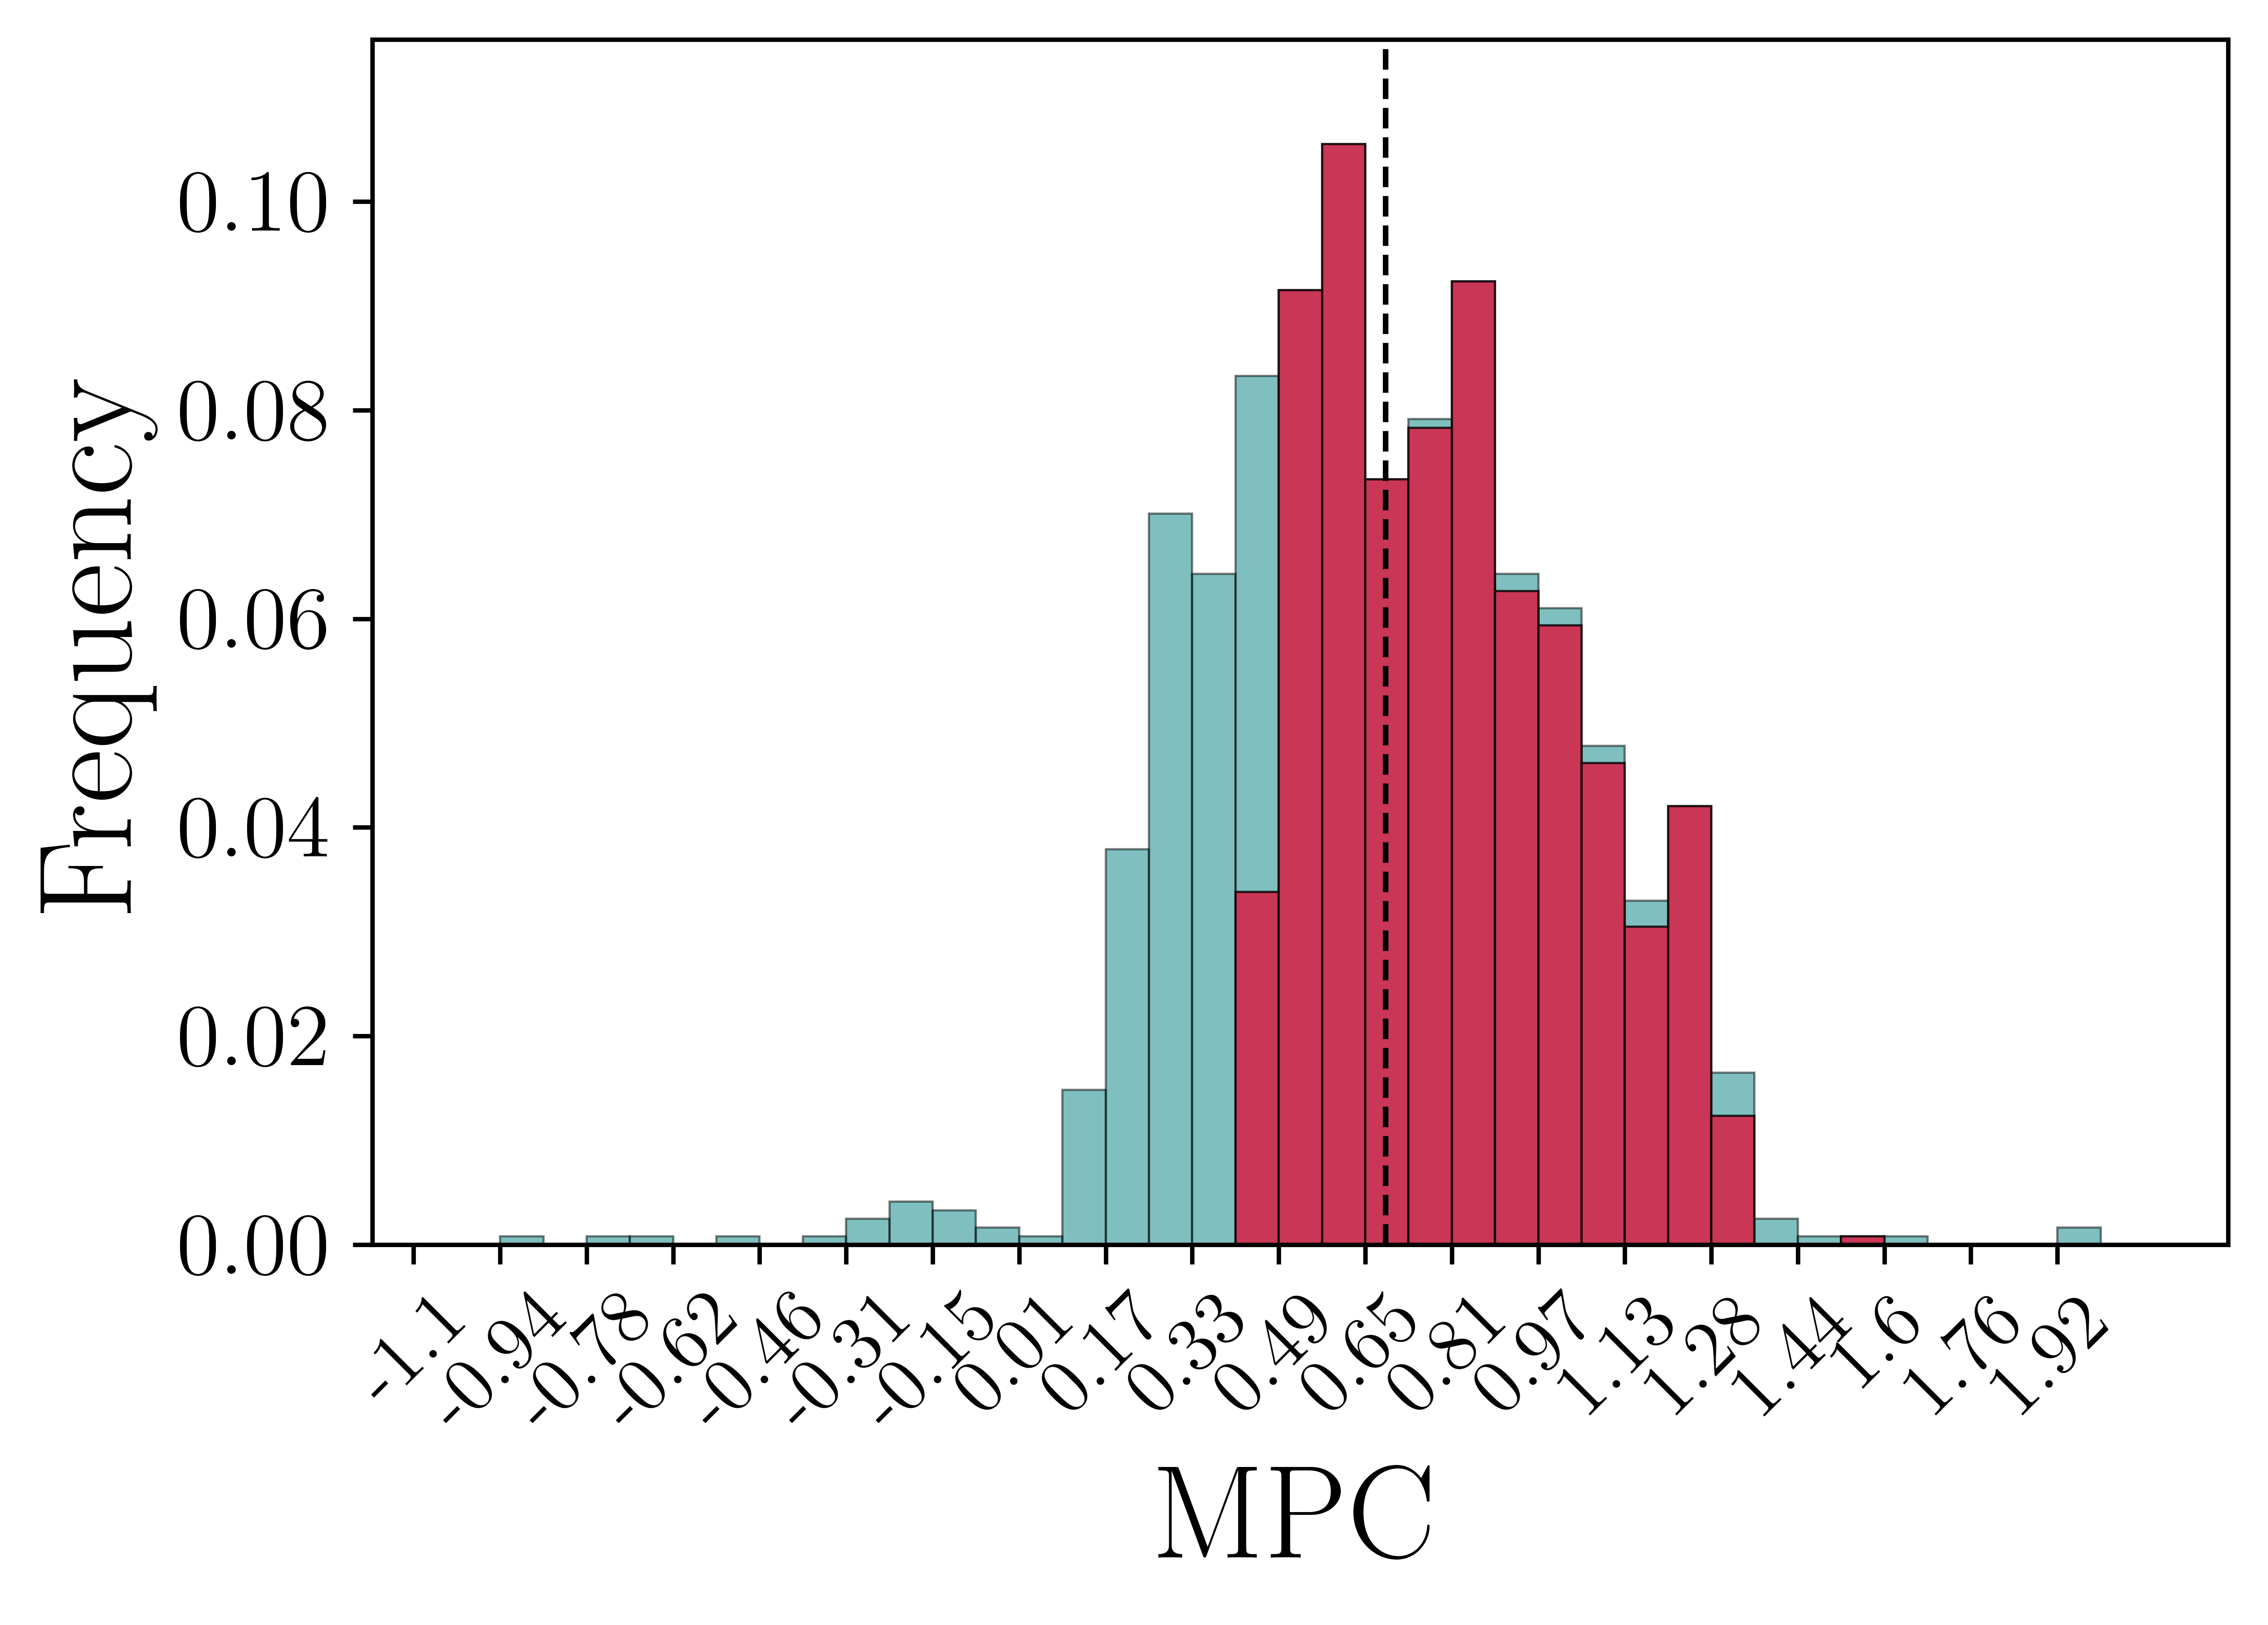
\includegraphics[width=\linewidth]{figures/distributions/spec1_lin_chTOTexp.png}
        \caption{Spec 1 - linear}
    \end{subfigure}\hfill
    \begin{subfigure}{0.33\linewidth}
        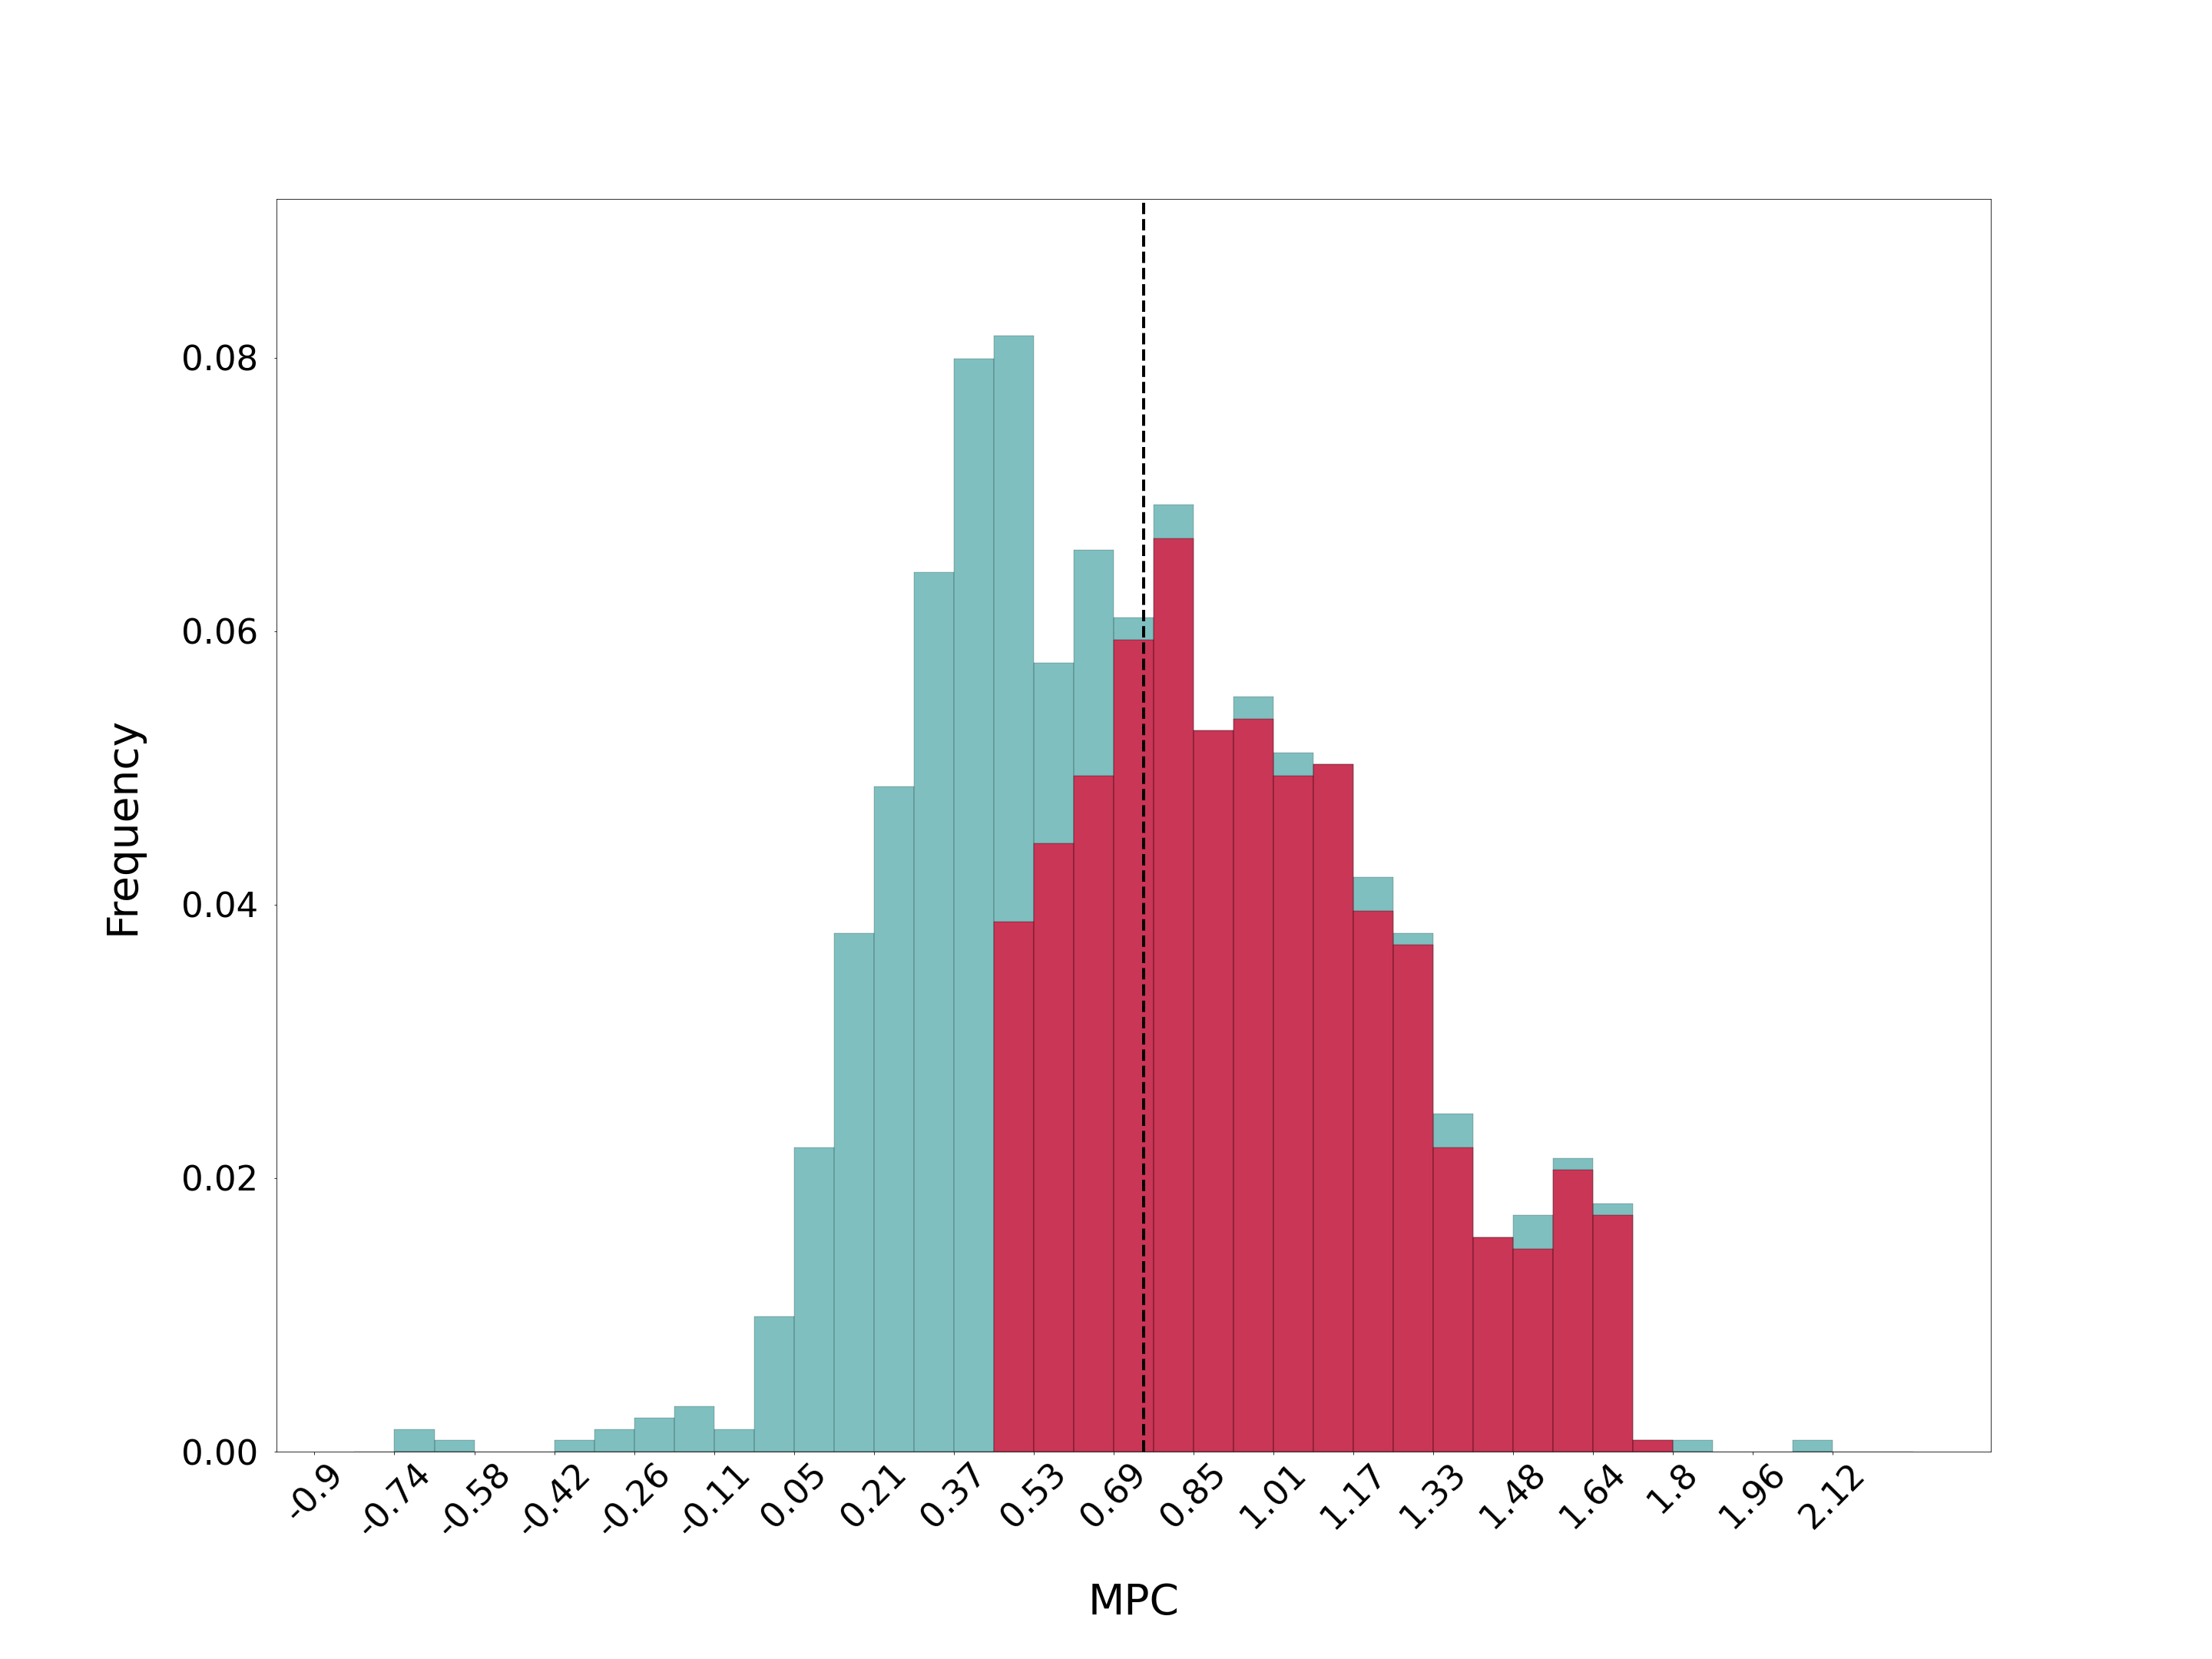
\includegraphics[width=\linewidth]{figures/distributions/spec2_lin_chTOTexp.png}
        \caption{Spec 2 - linear}
    \end{subfigure}\hfill
    \begin{subfigure}{0.33\linewidth}
        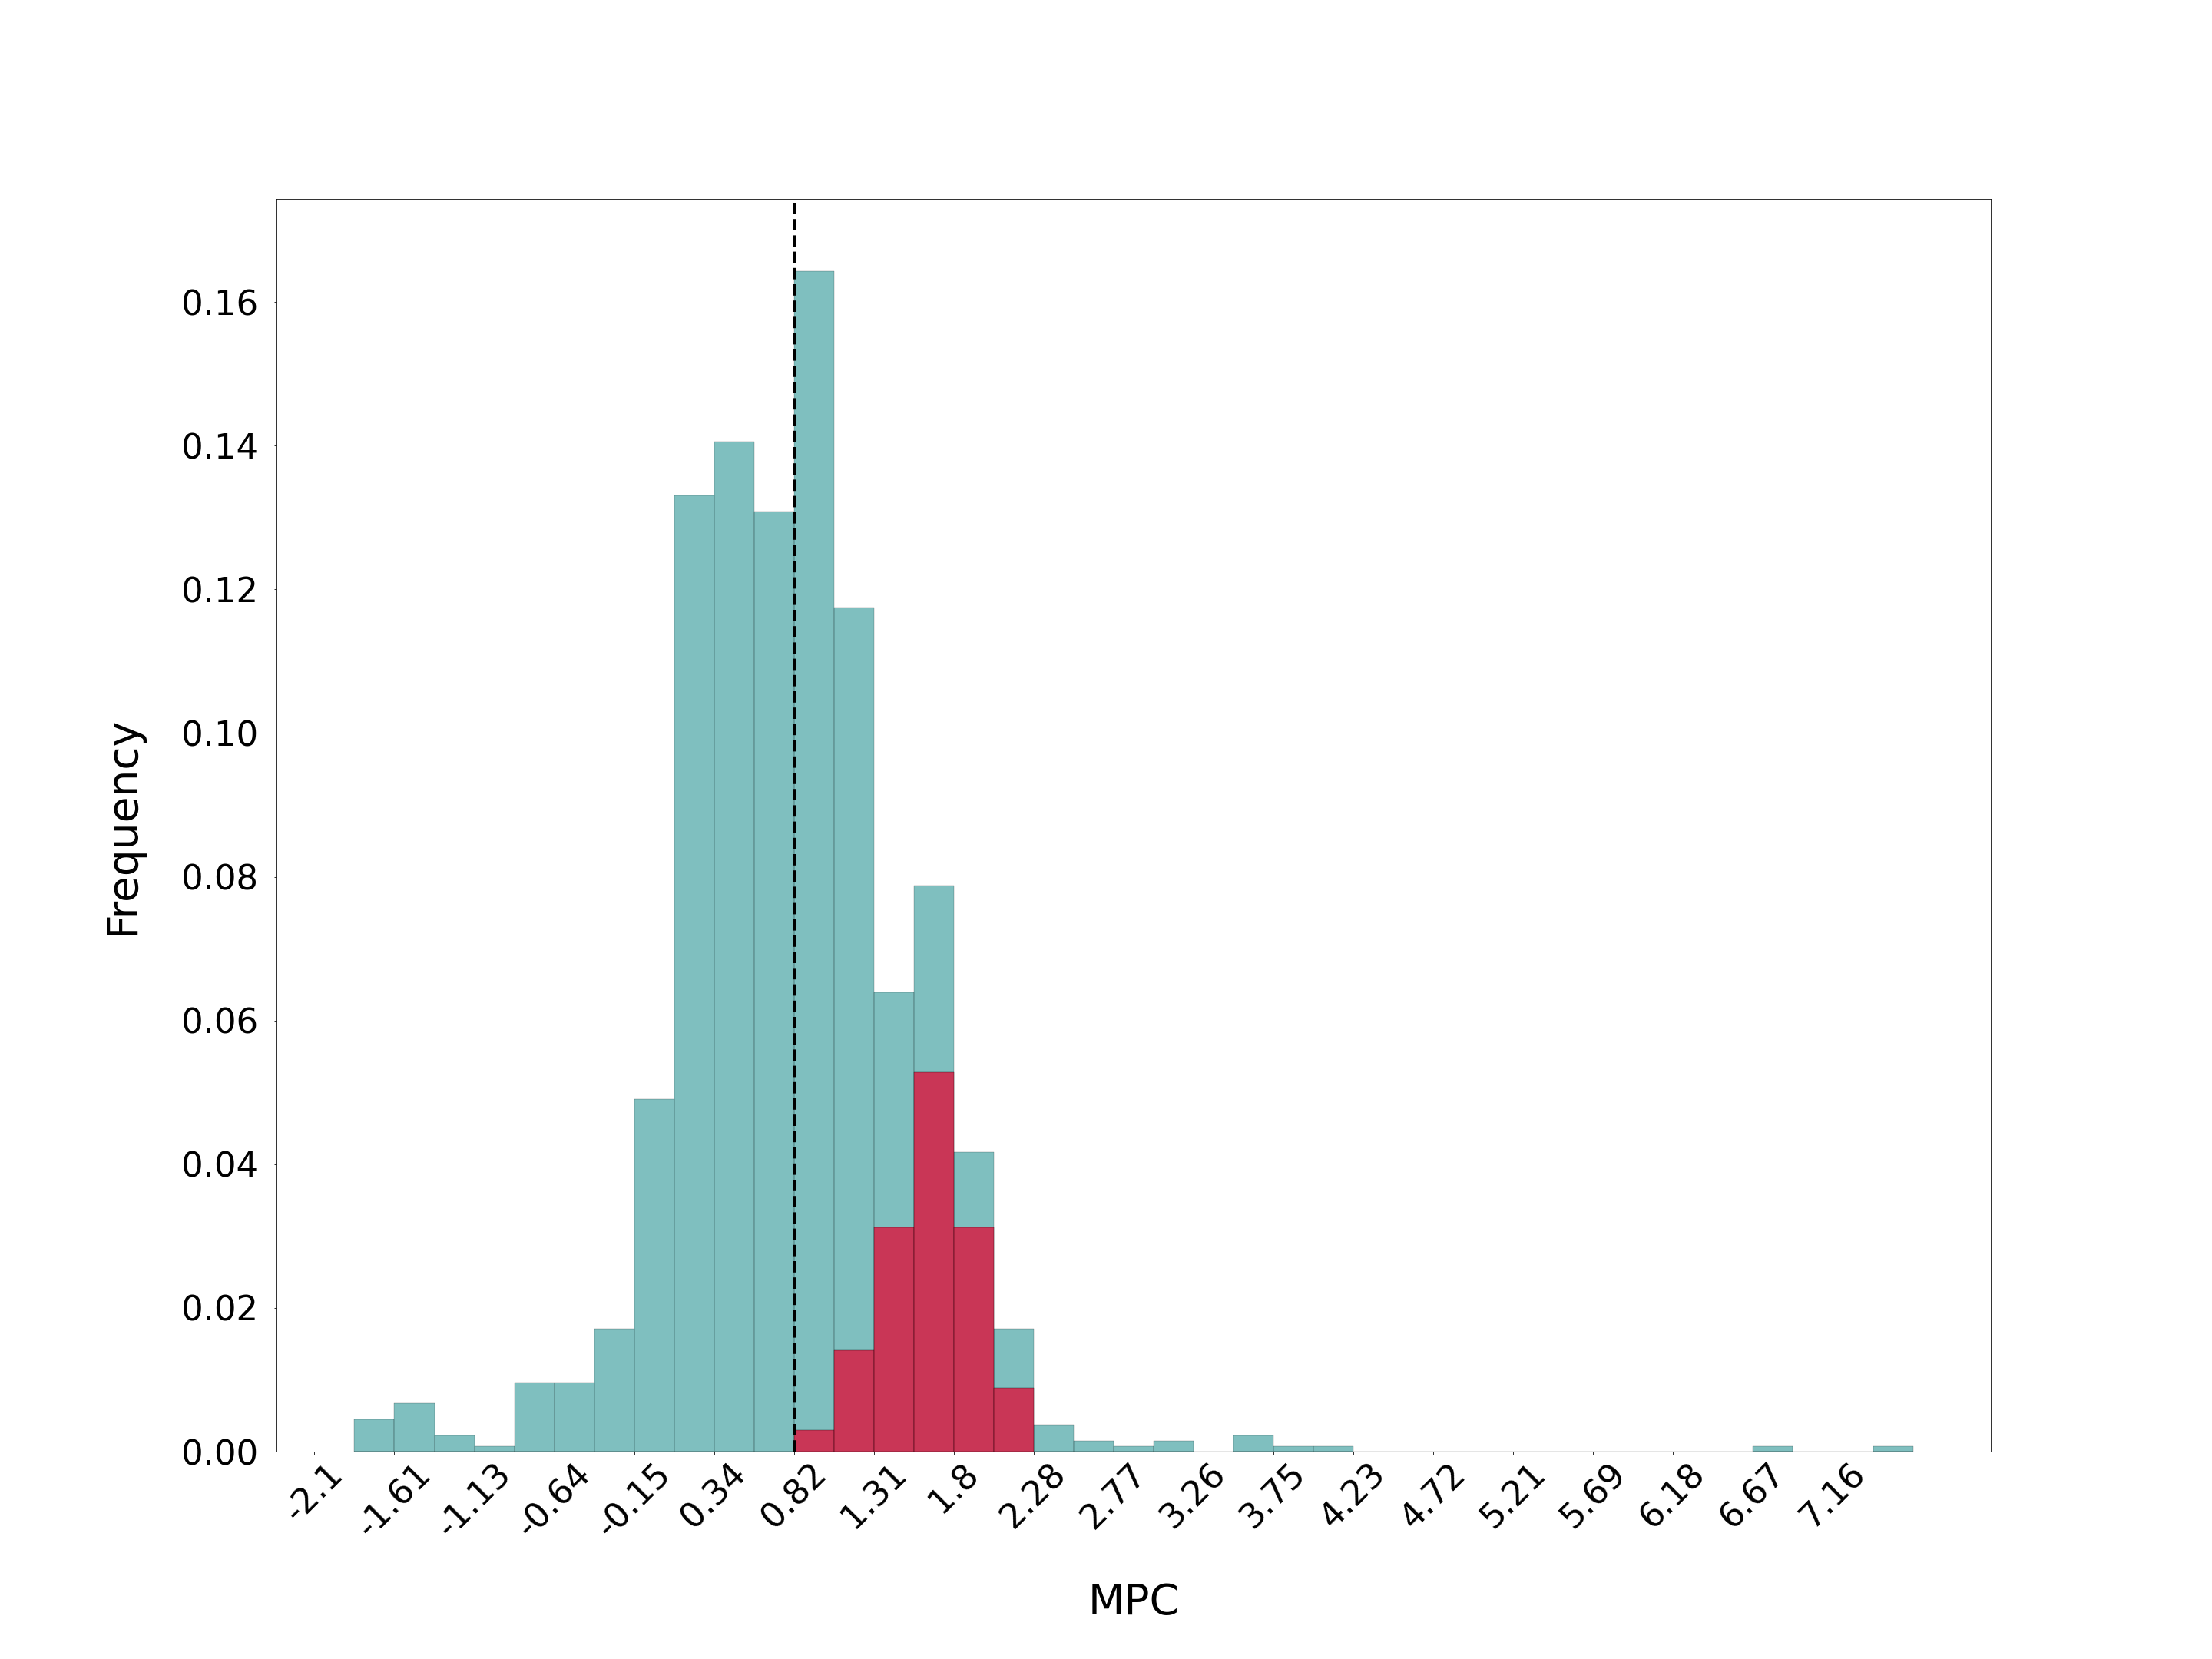
\includegraphics[width=\linewidth]{figures/distributions/spec3_lin_chTOTexp.png}
        \caption{Spec 3 - linear}
    \end{subfigure}\hfill
    
%    \mbox{}\hfill
    \begin{subfigure}{0.33\linewidth}
        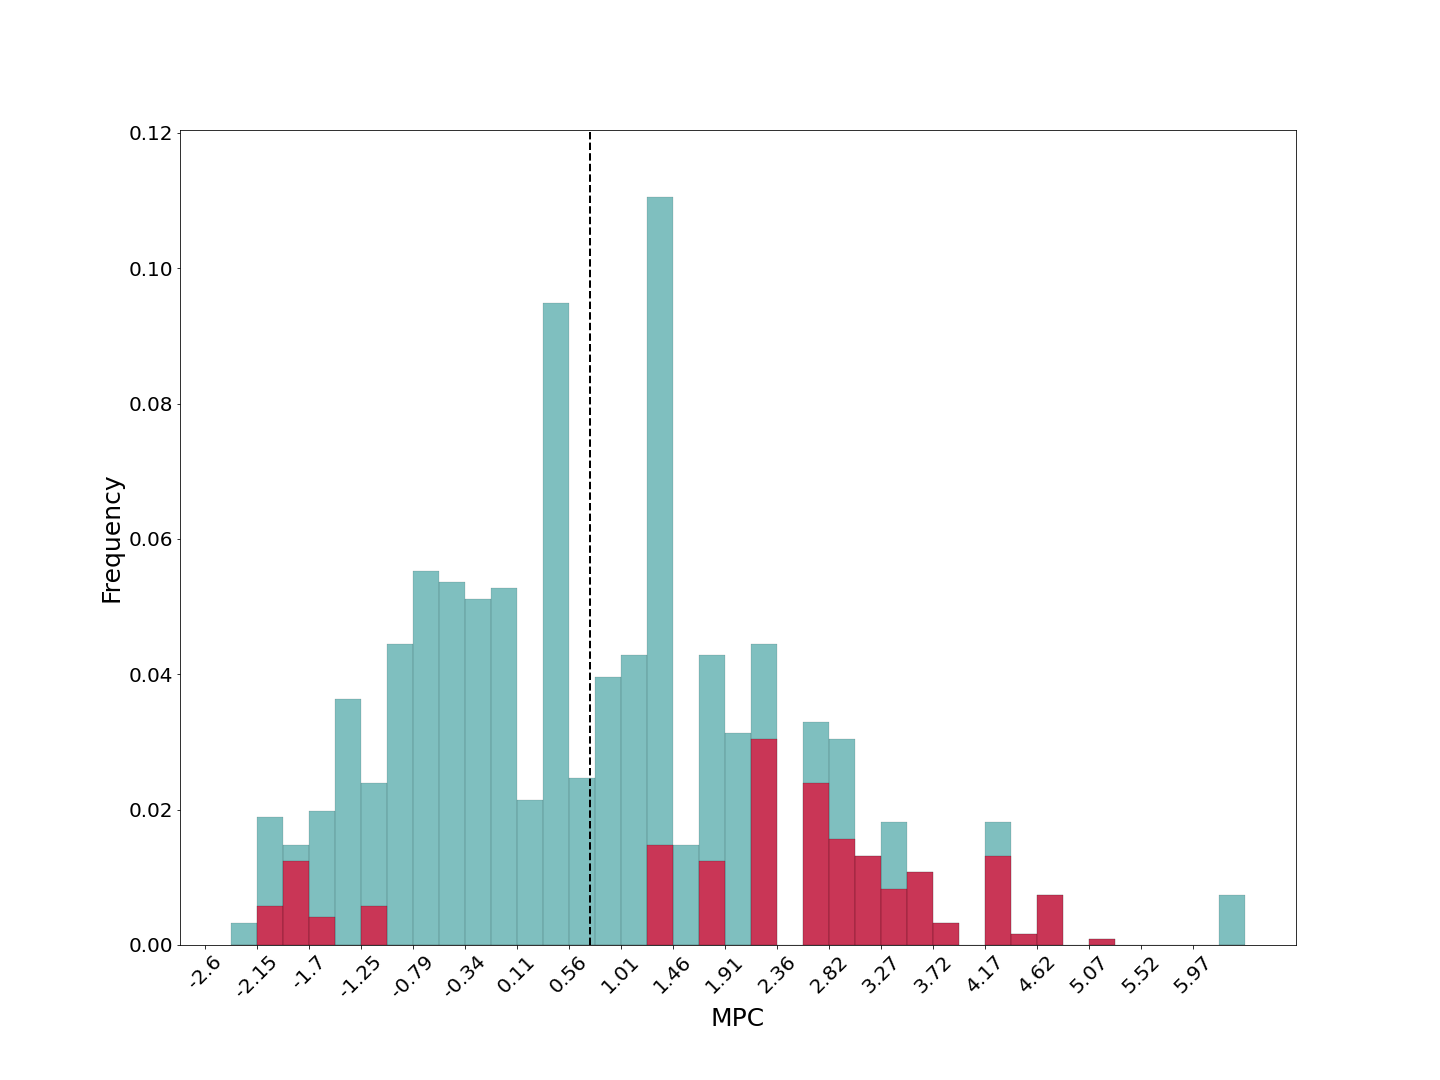
\includegraphics[width=\linewidth]{figures/distributions/spec1_cf_chTOTexp.png}
        \caption{Spec 1 - causal forest}
    \end{subfigure}\hfill
    \begin{subfigure}{0.33\linewidth}
        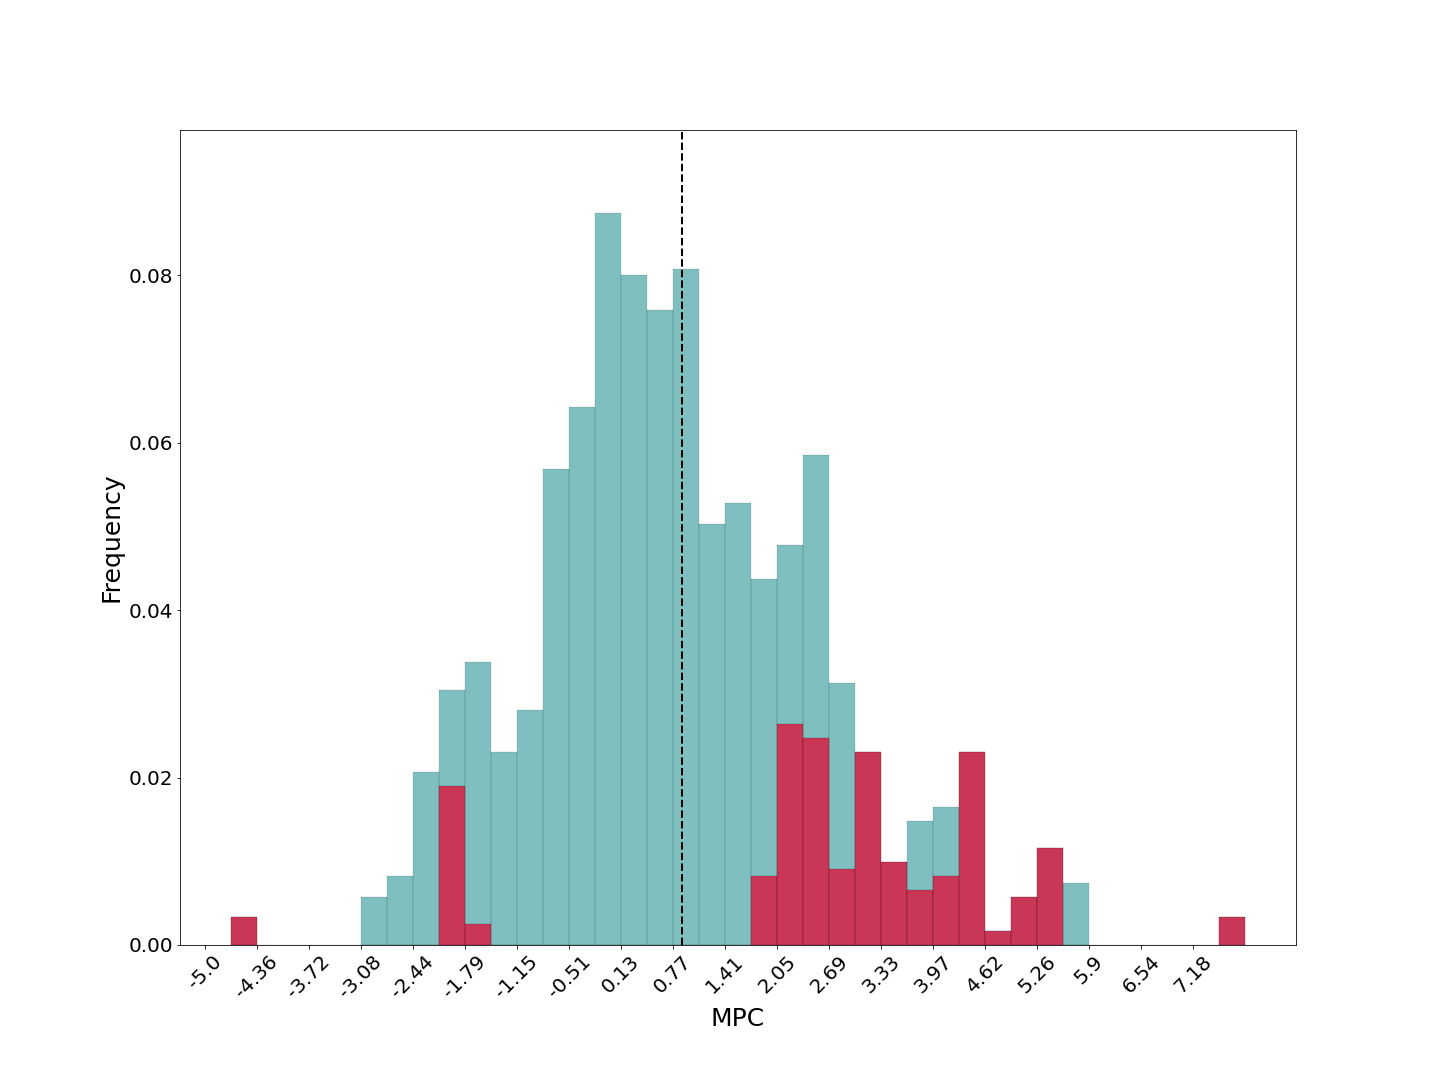
\includegraphics[width=\linewidth]{figures/distributions/spec2_cf_chTOTexp.png}
        \caption{Spec 2 - causal forest}
    \end{subfigure}\hfill
    \begin{subfigure}{0.33\linewidth}
        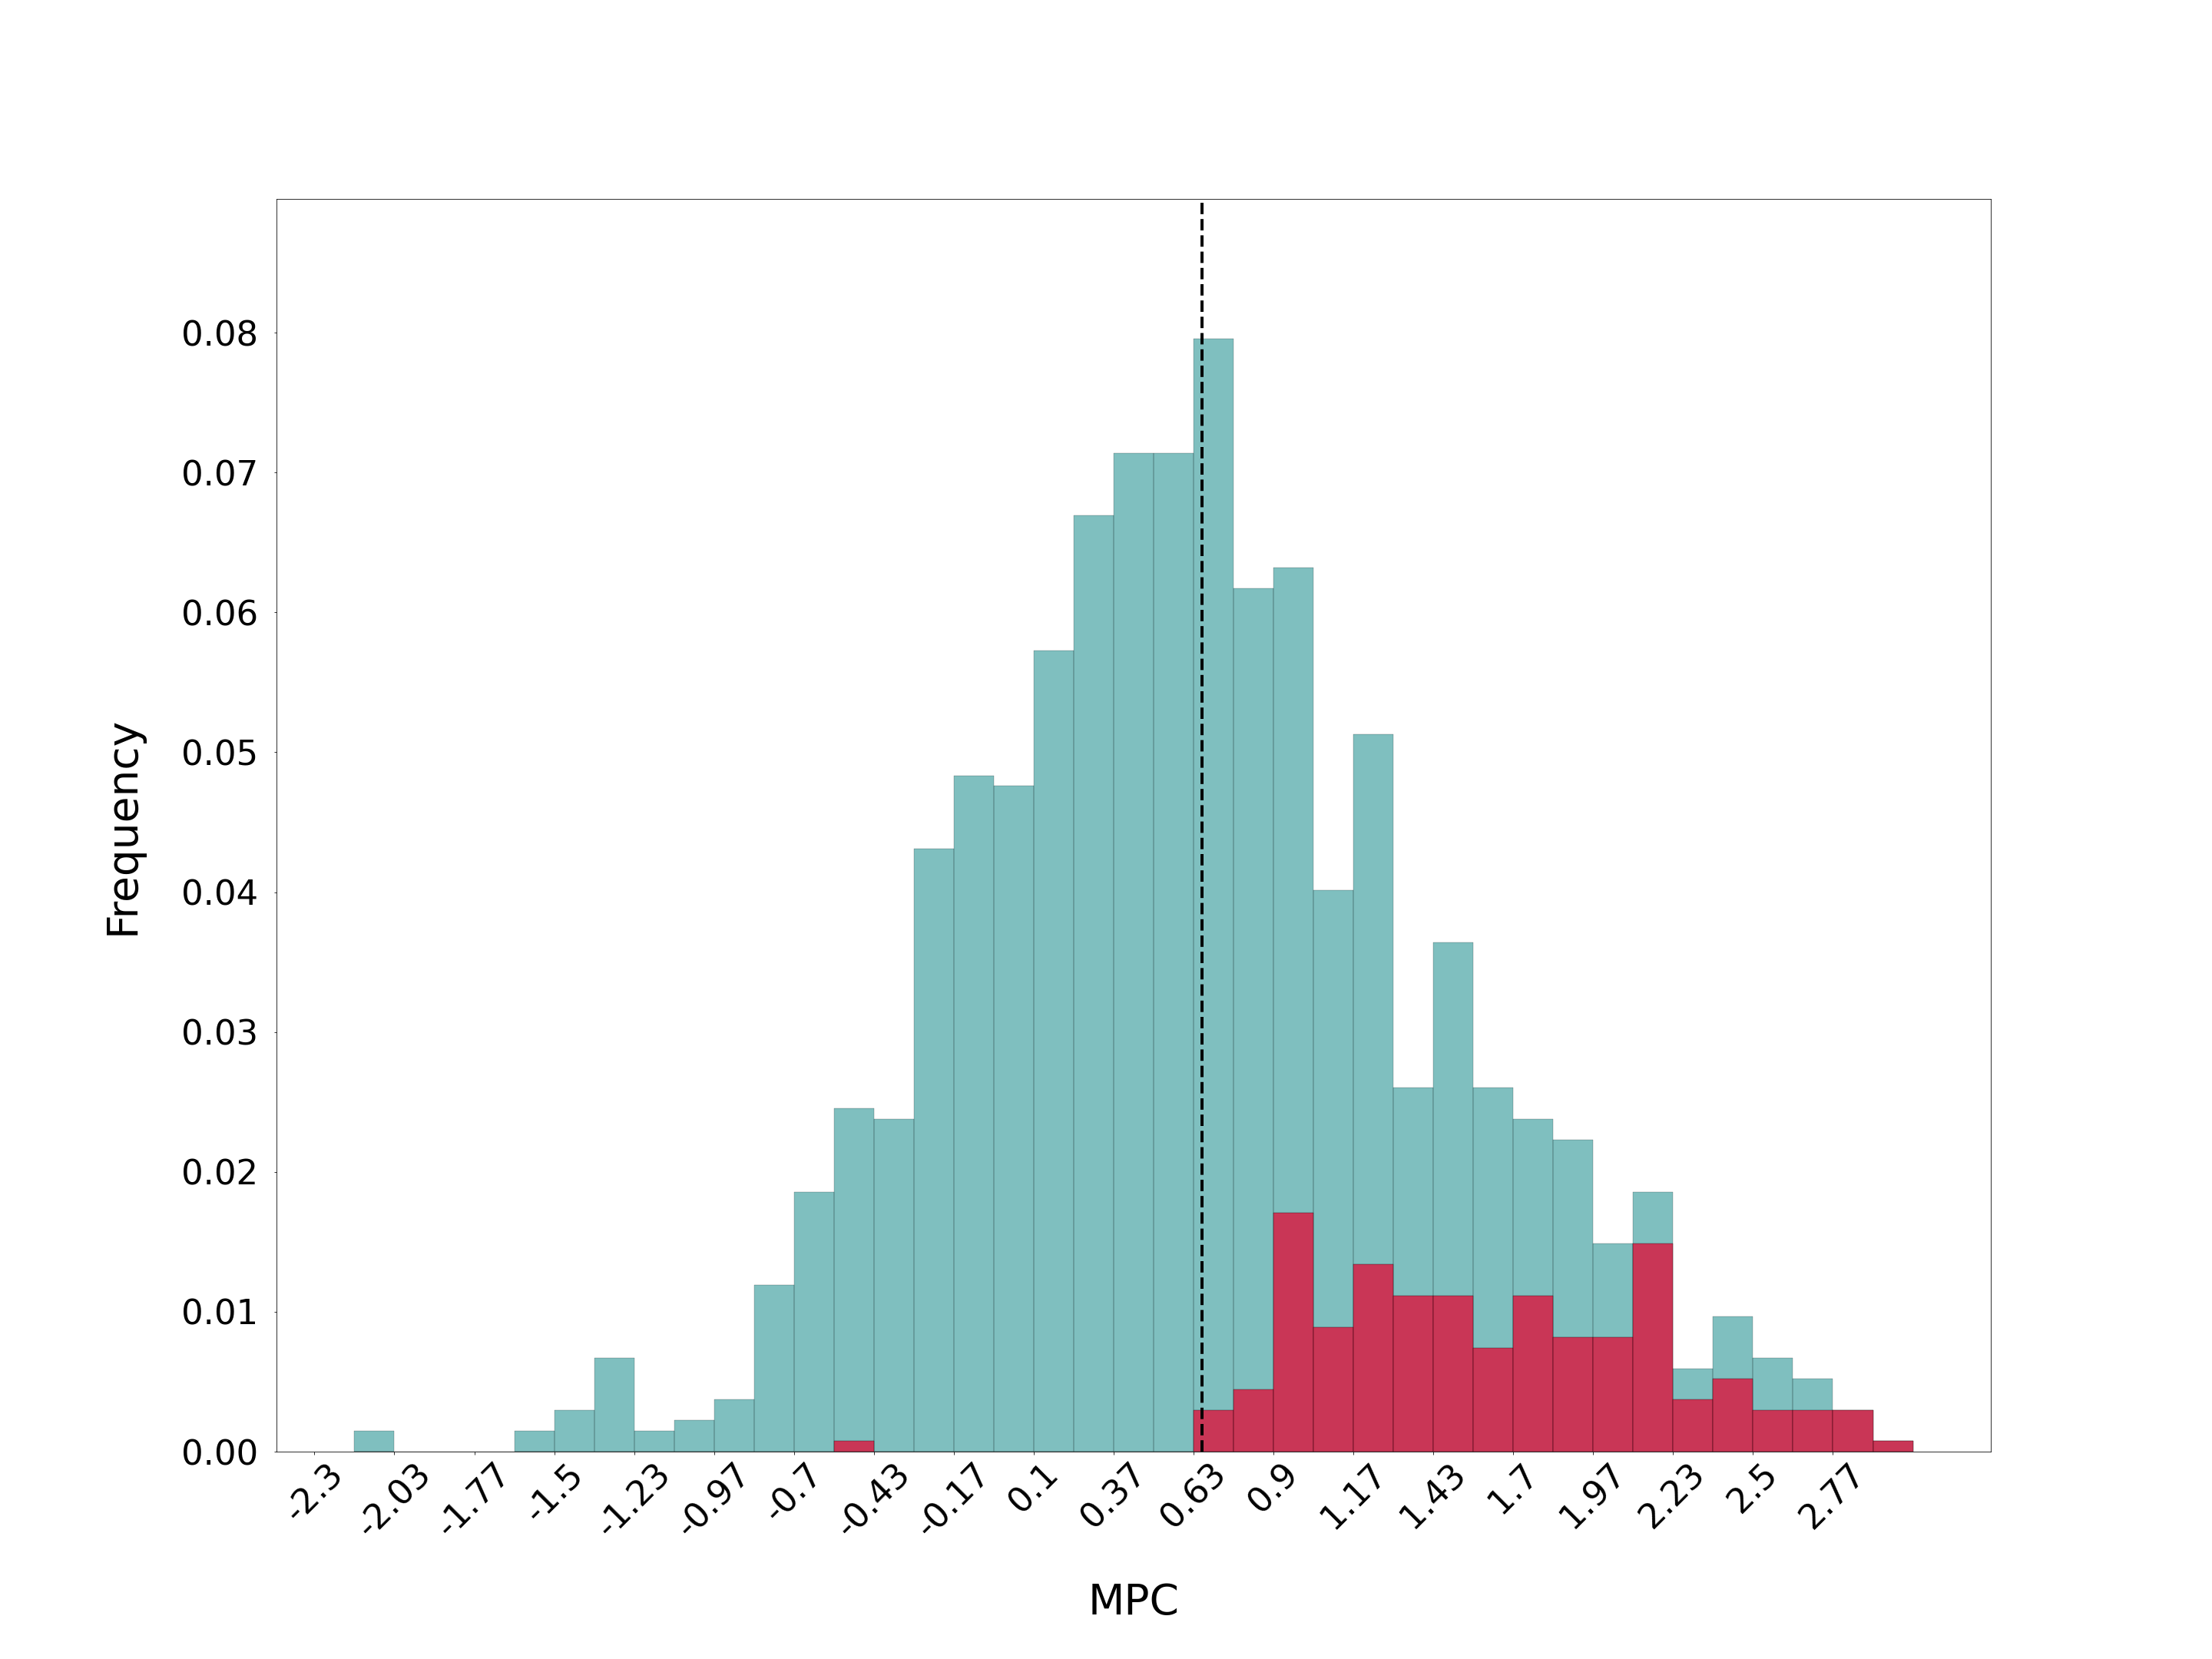
\includegraphics[width=\linewidth]{figures/distributions/spec3_cf_chTOTexp.png}
        \caption{Spec 3 - causal forest}
    \end{subfigure}\hfill
    \fnote{Blue parts show frequency of point estimates in this bin, red parts show share of these being statistically significant with $p\leq0.1$. Dotted lines signal the \textit{Average Treatment Effect}.}
    \caption{Distributions of estimated MPC - total expenditures}
    \label{fig:dist_tot}
\end{figure}
\begin{figure}[t]
    \centering
%    \mbox{}\hfill
    \begin{subfigure}{0.33\linewidth}
        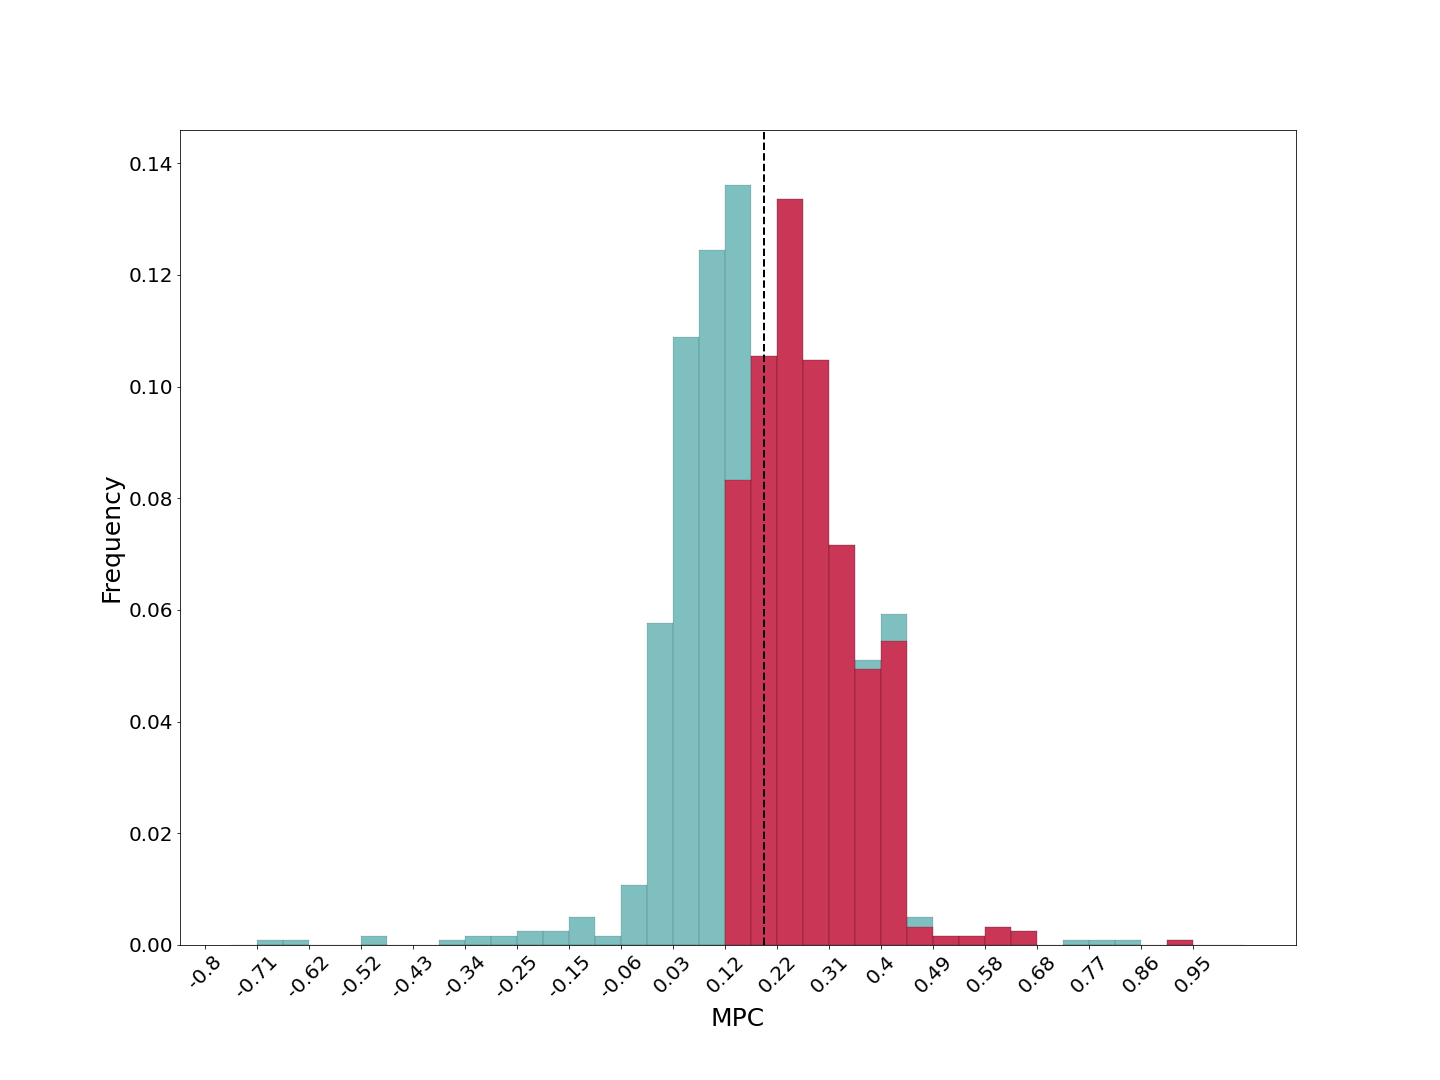
\includegraphics[width=\linewidth]{figures/distributions/spec1_lin_chNDexp.png}
        \caption{Spec 1 - linear}
    \end{subfigure}\hfill
    \begin{subfigure}{0.33\linewidth}
        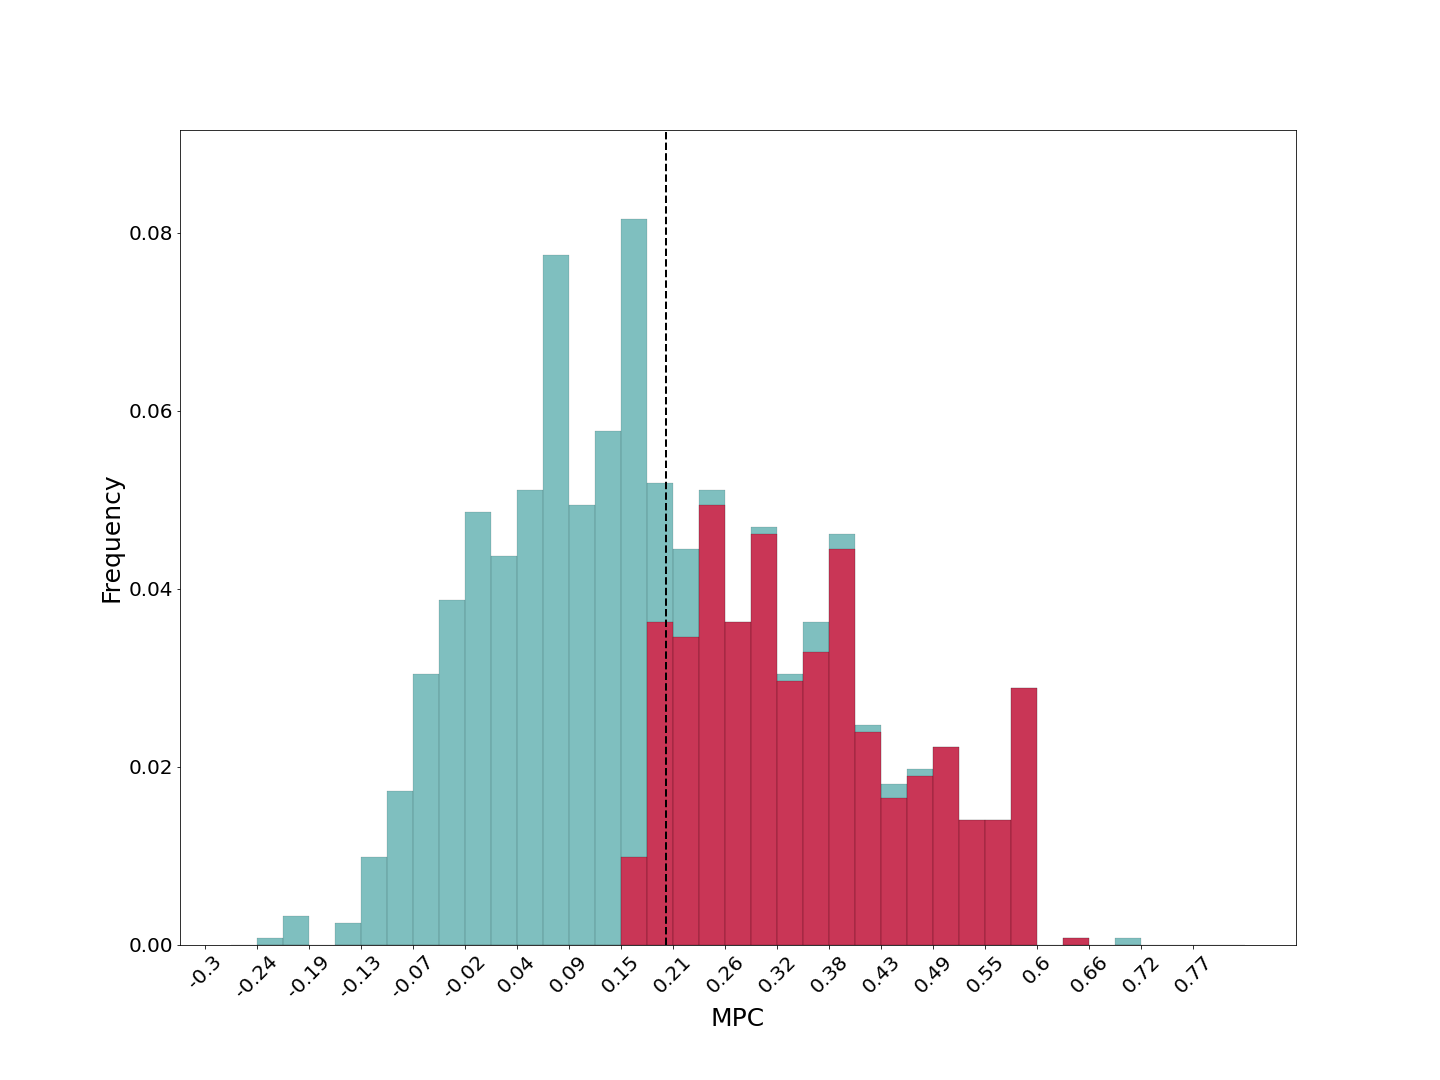
\includegraphics[width=\linewidth]{figures/distributions/spec2_lin_chNDexp.png}
        \caption{Spec 2 - linear}
    \end{subfigure}\hfill
    \begin{subfigure}{0.33\linewidth}
        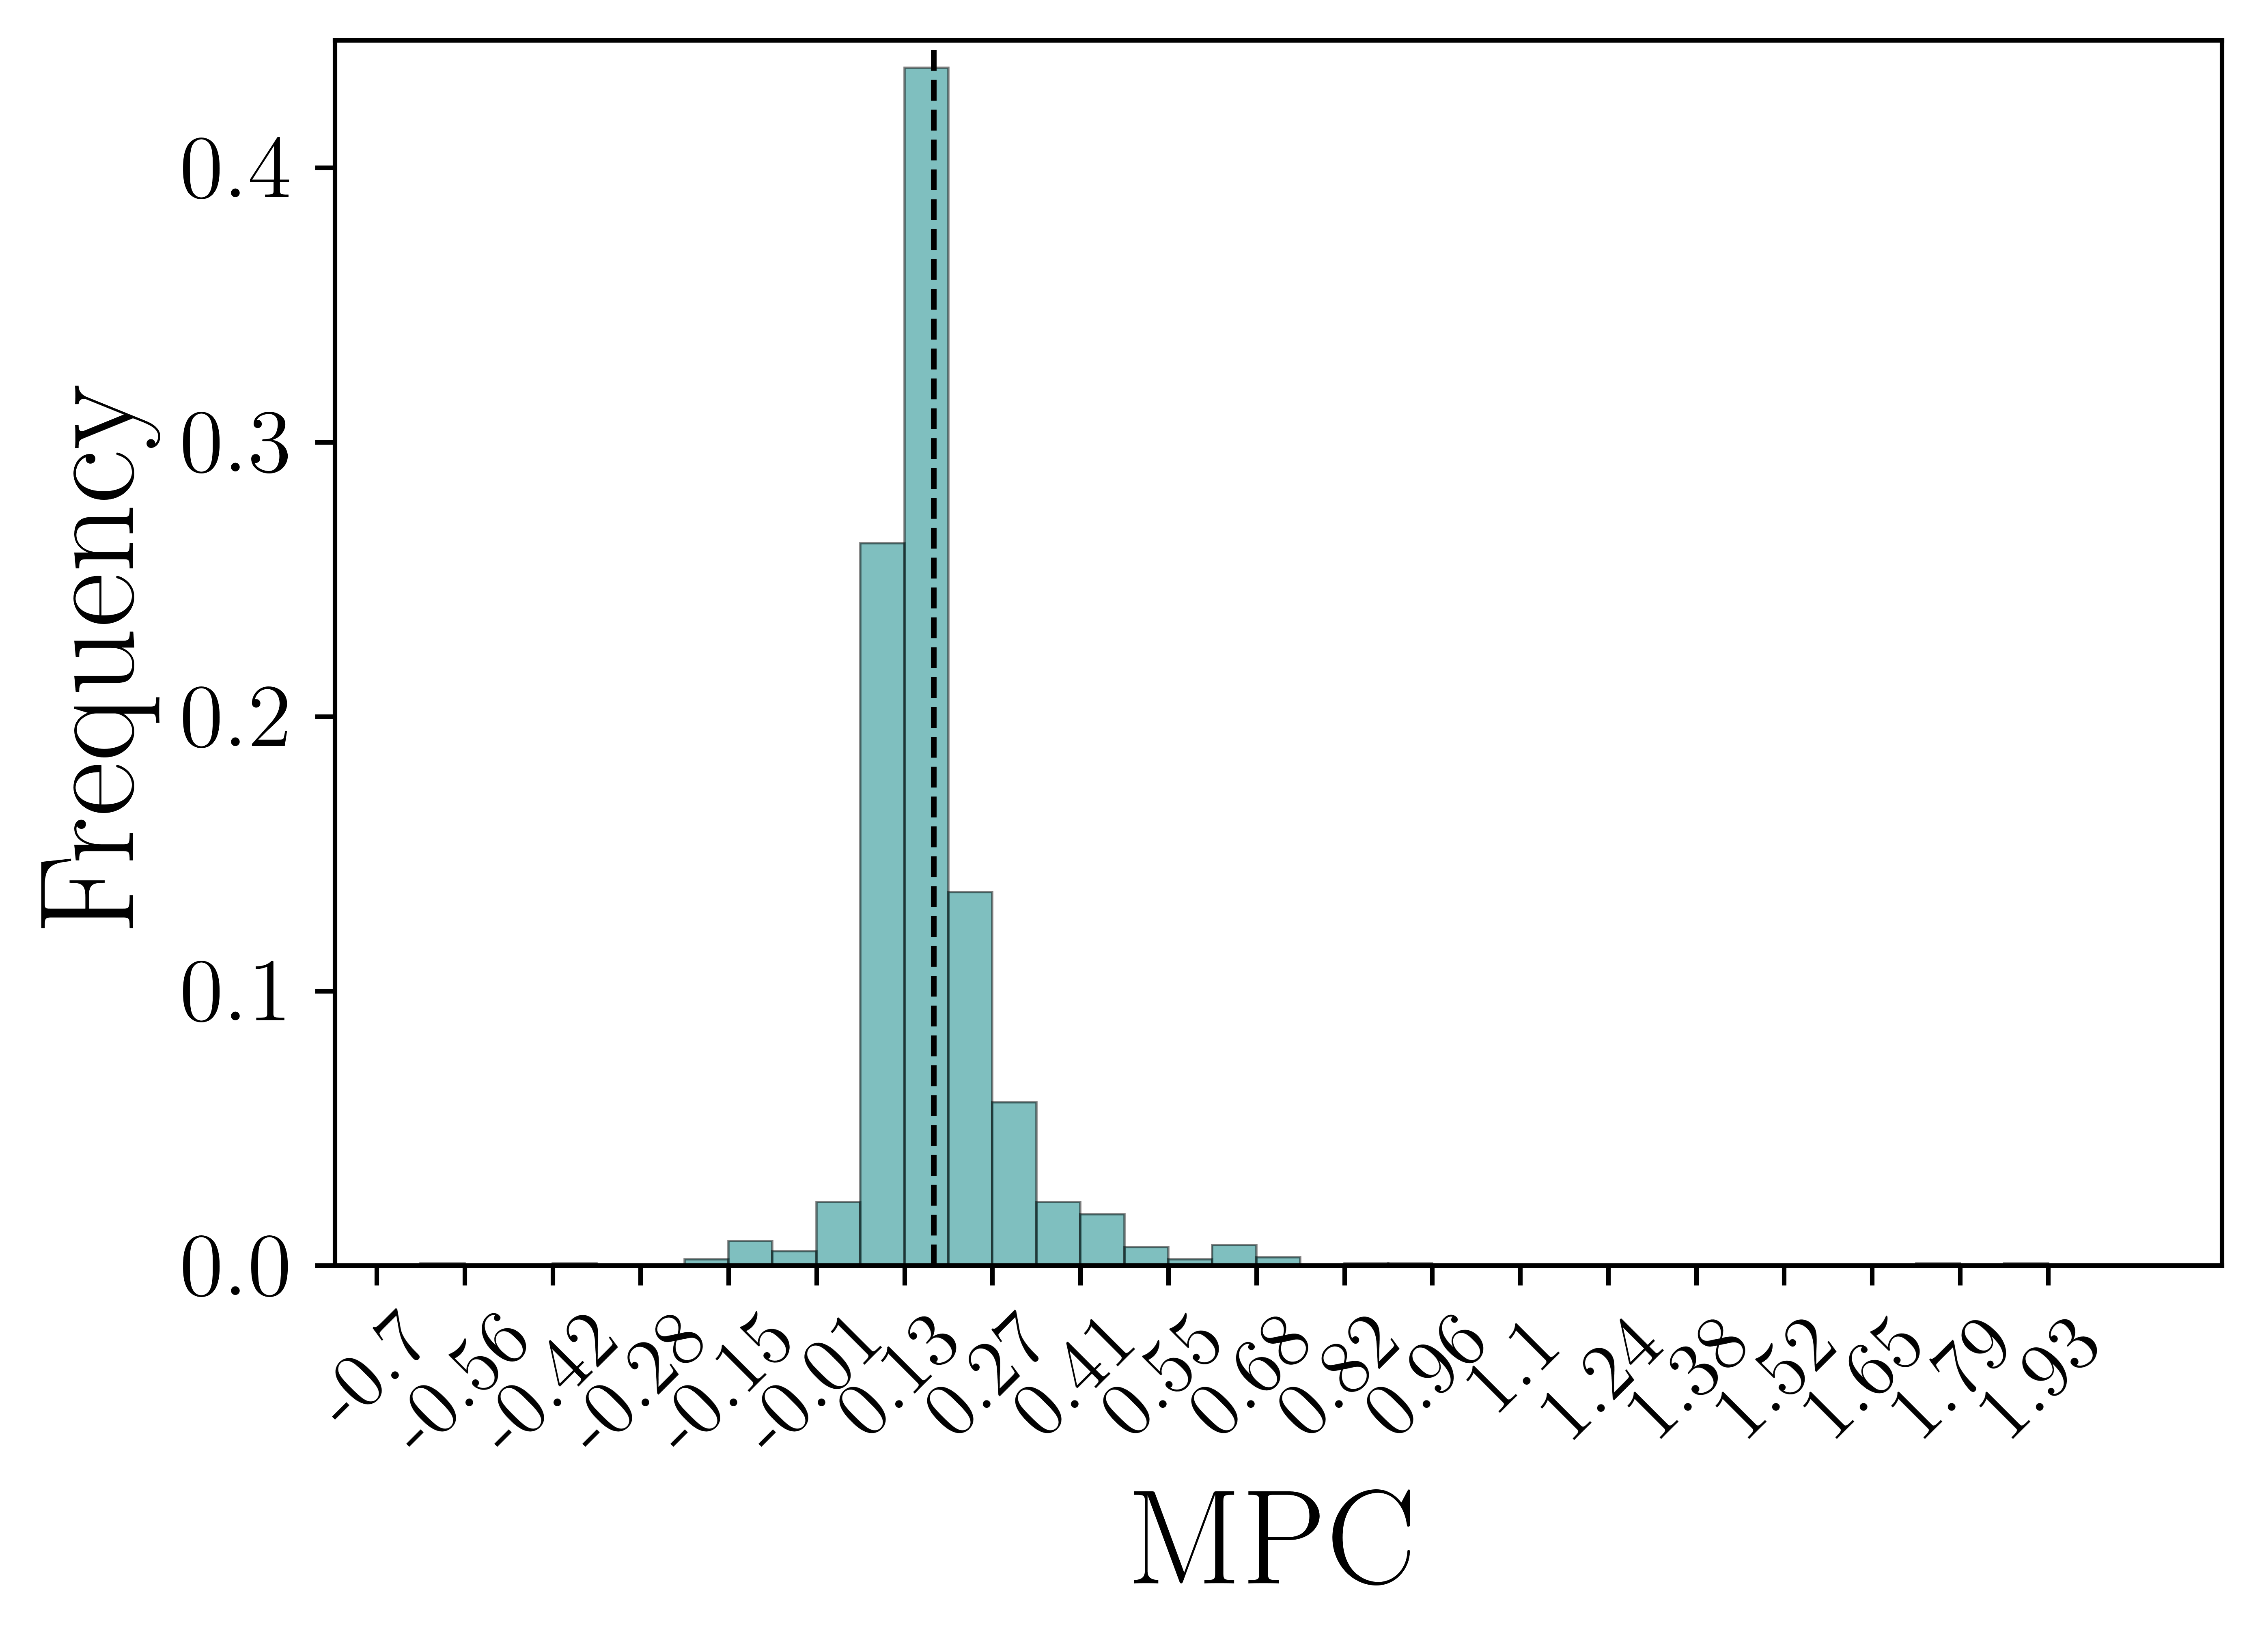
\includegraphics[width=\linewidth]{figures/distributions/spec3_lin_chNDexp.png}
        \caption{Spec 3 - linear}
    \end{subfigure}\hfill
    
%    \mbox{}\hfill
    \begin{subfigure}{0.33\linewidth}
        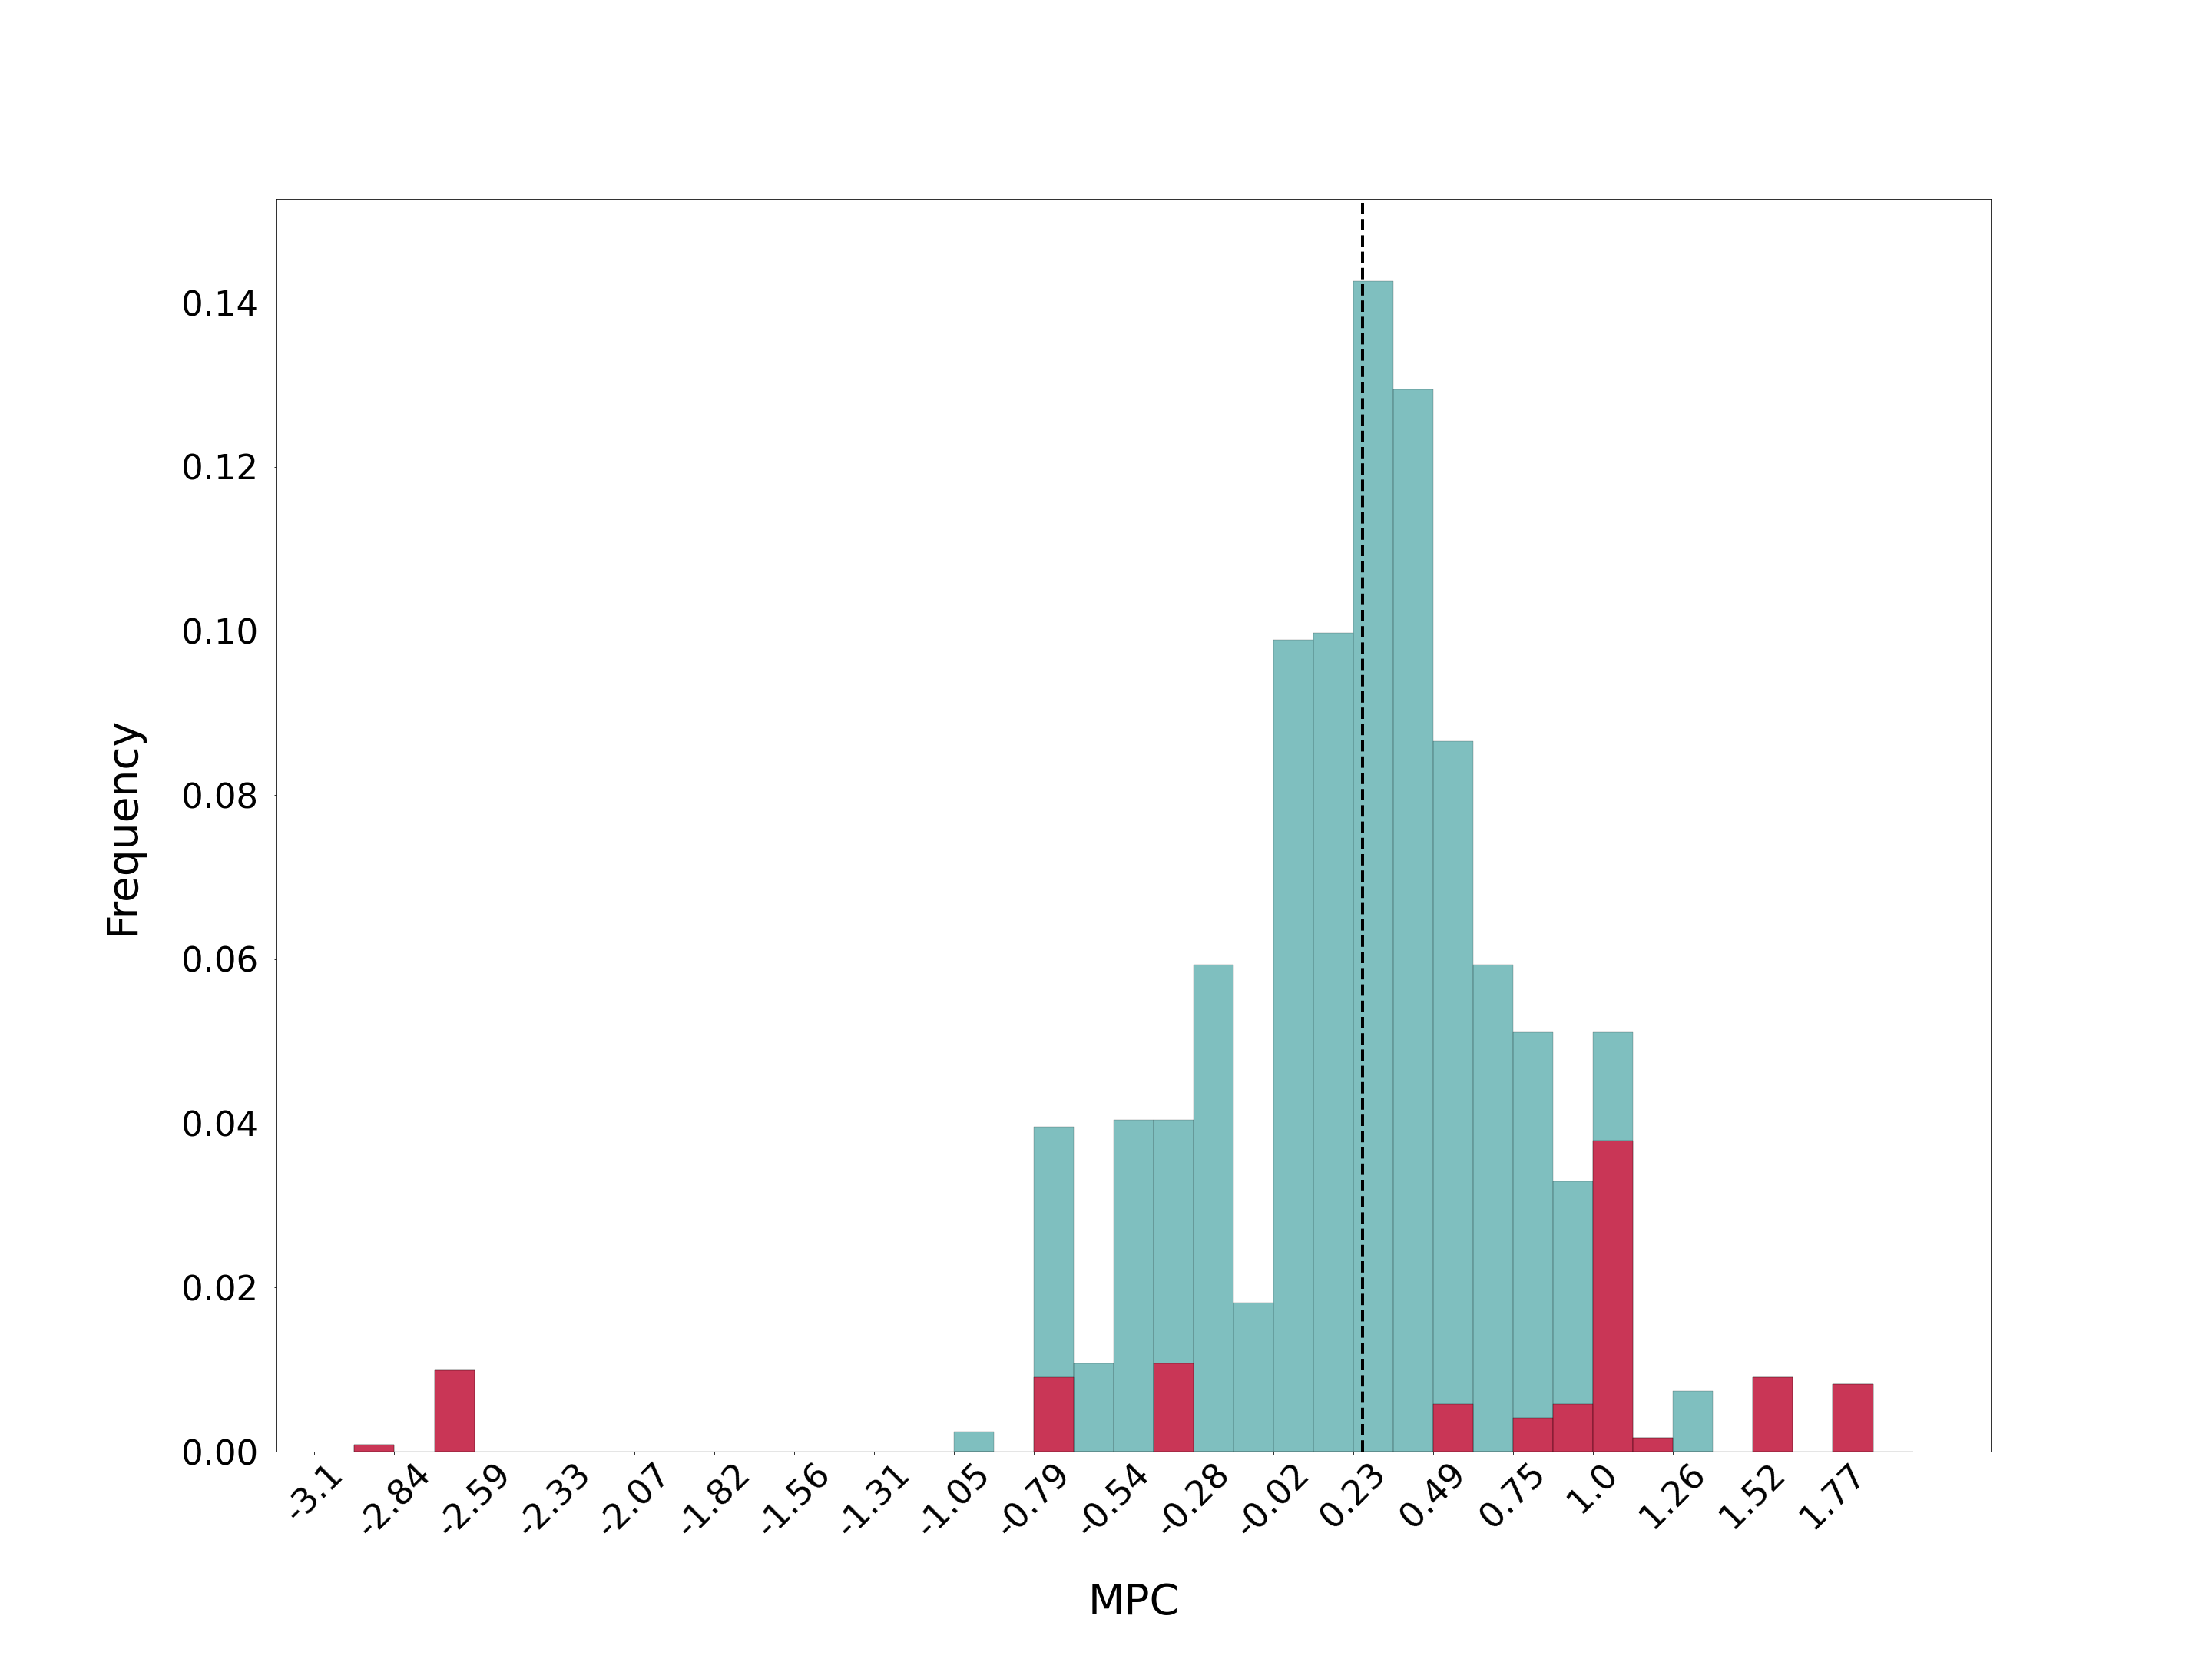
\includegraphics[width=\linewidth]{figures/distributions/spec1_cf_chNDexp.png}
        \caption{Spec 1 - causal forest}
    \end{subfigure}\hfill
    \begin{subfigure}{0.33\linewidth}
        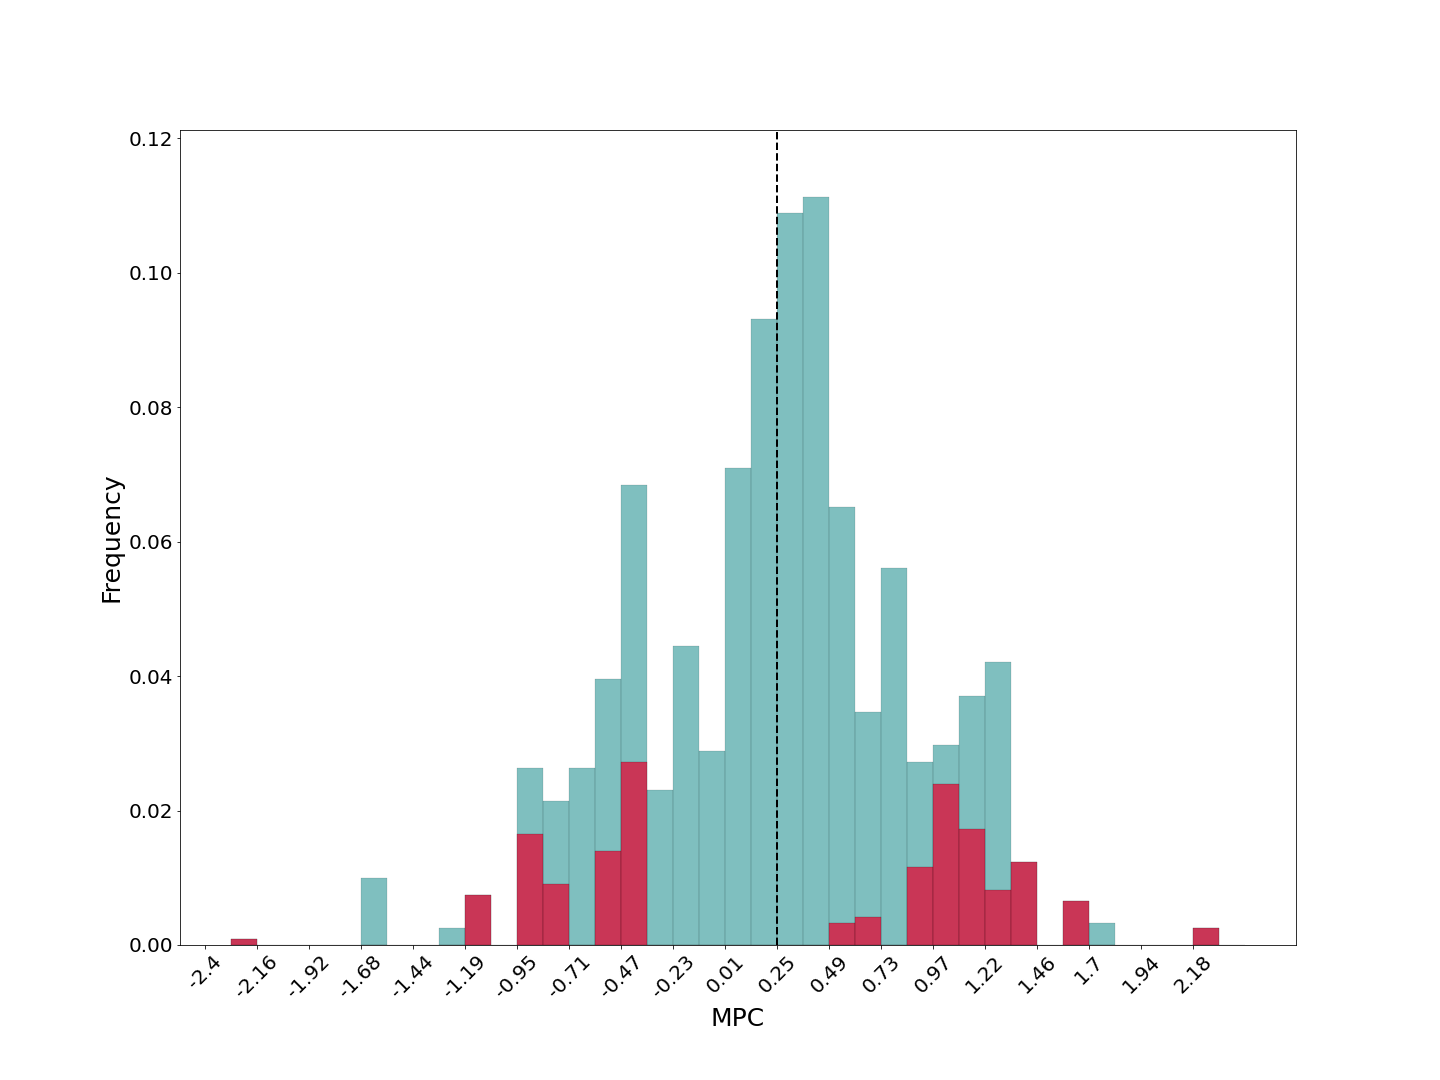
\includegraphics[width=\linewidth]{figures/distributions/spec2_cf_chNDexp.png}
        \caption{Spec 2 - causal forest}
    \end{subfigure}\hfill
    \begin{subfigure}{0.33\linewidth}
        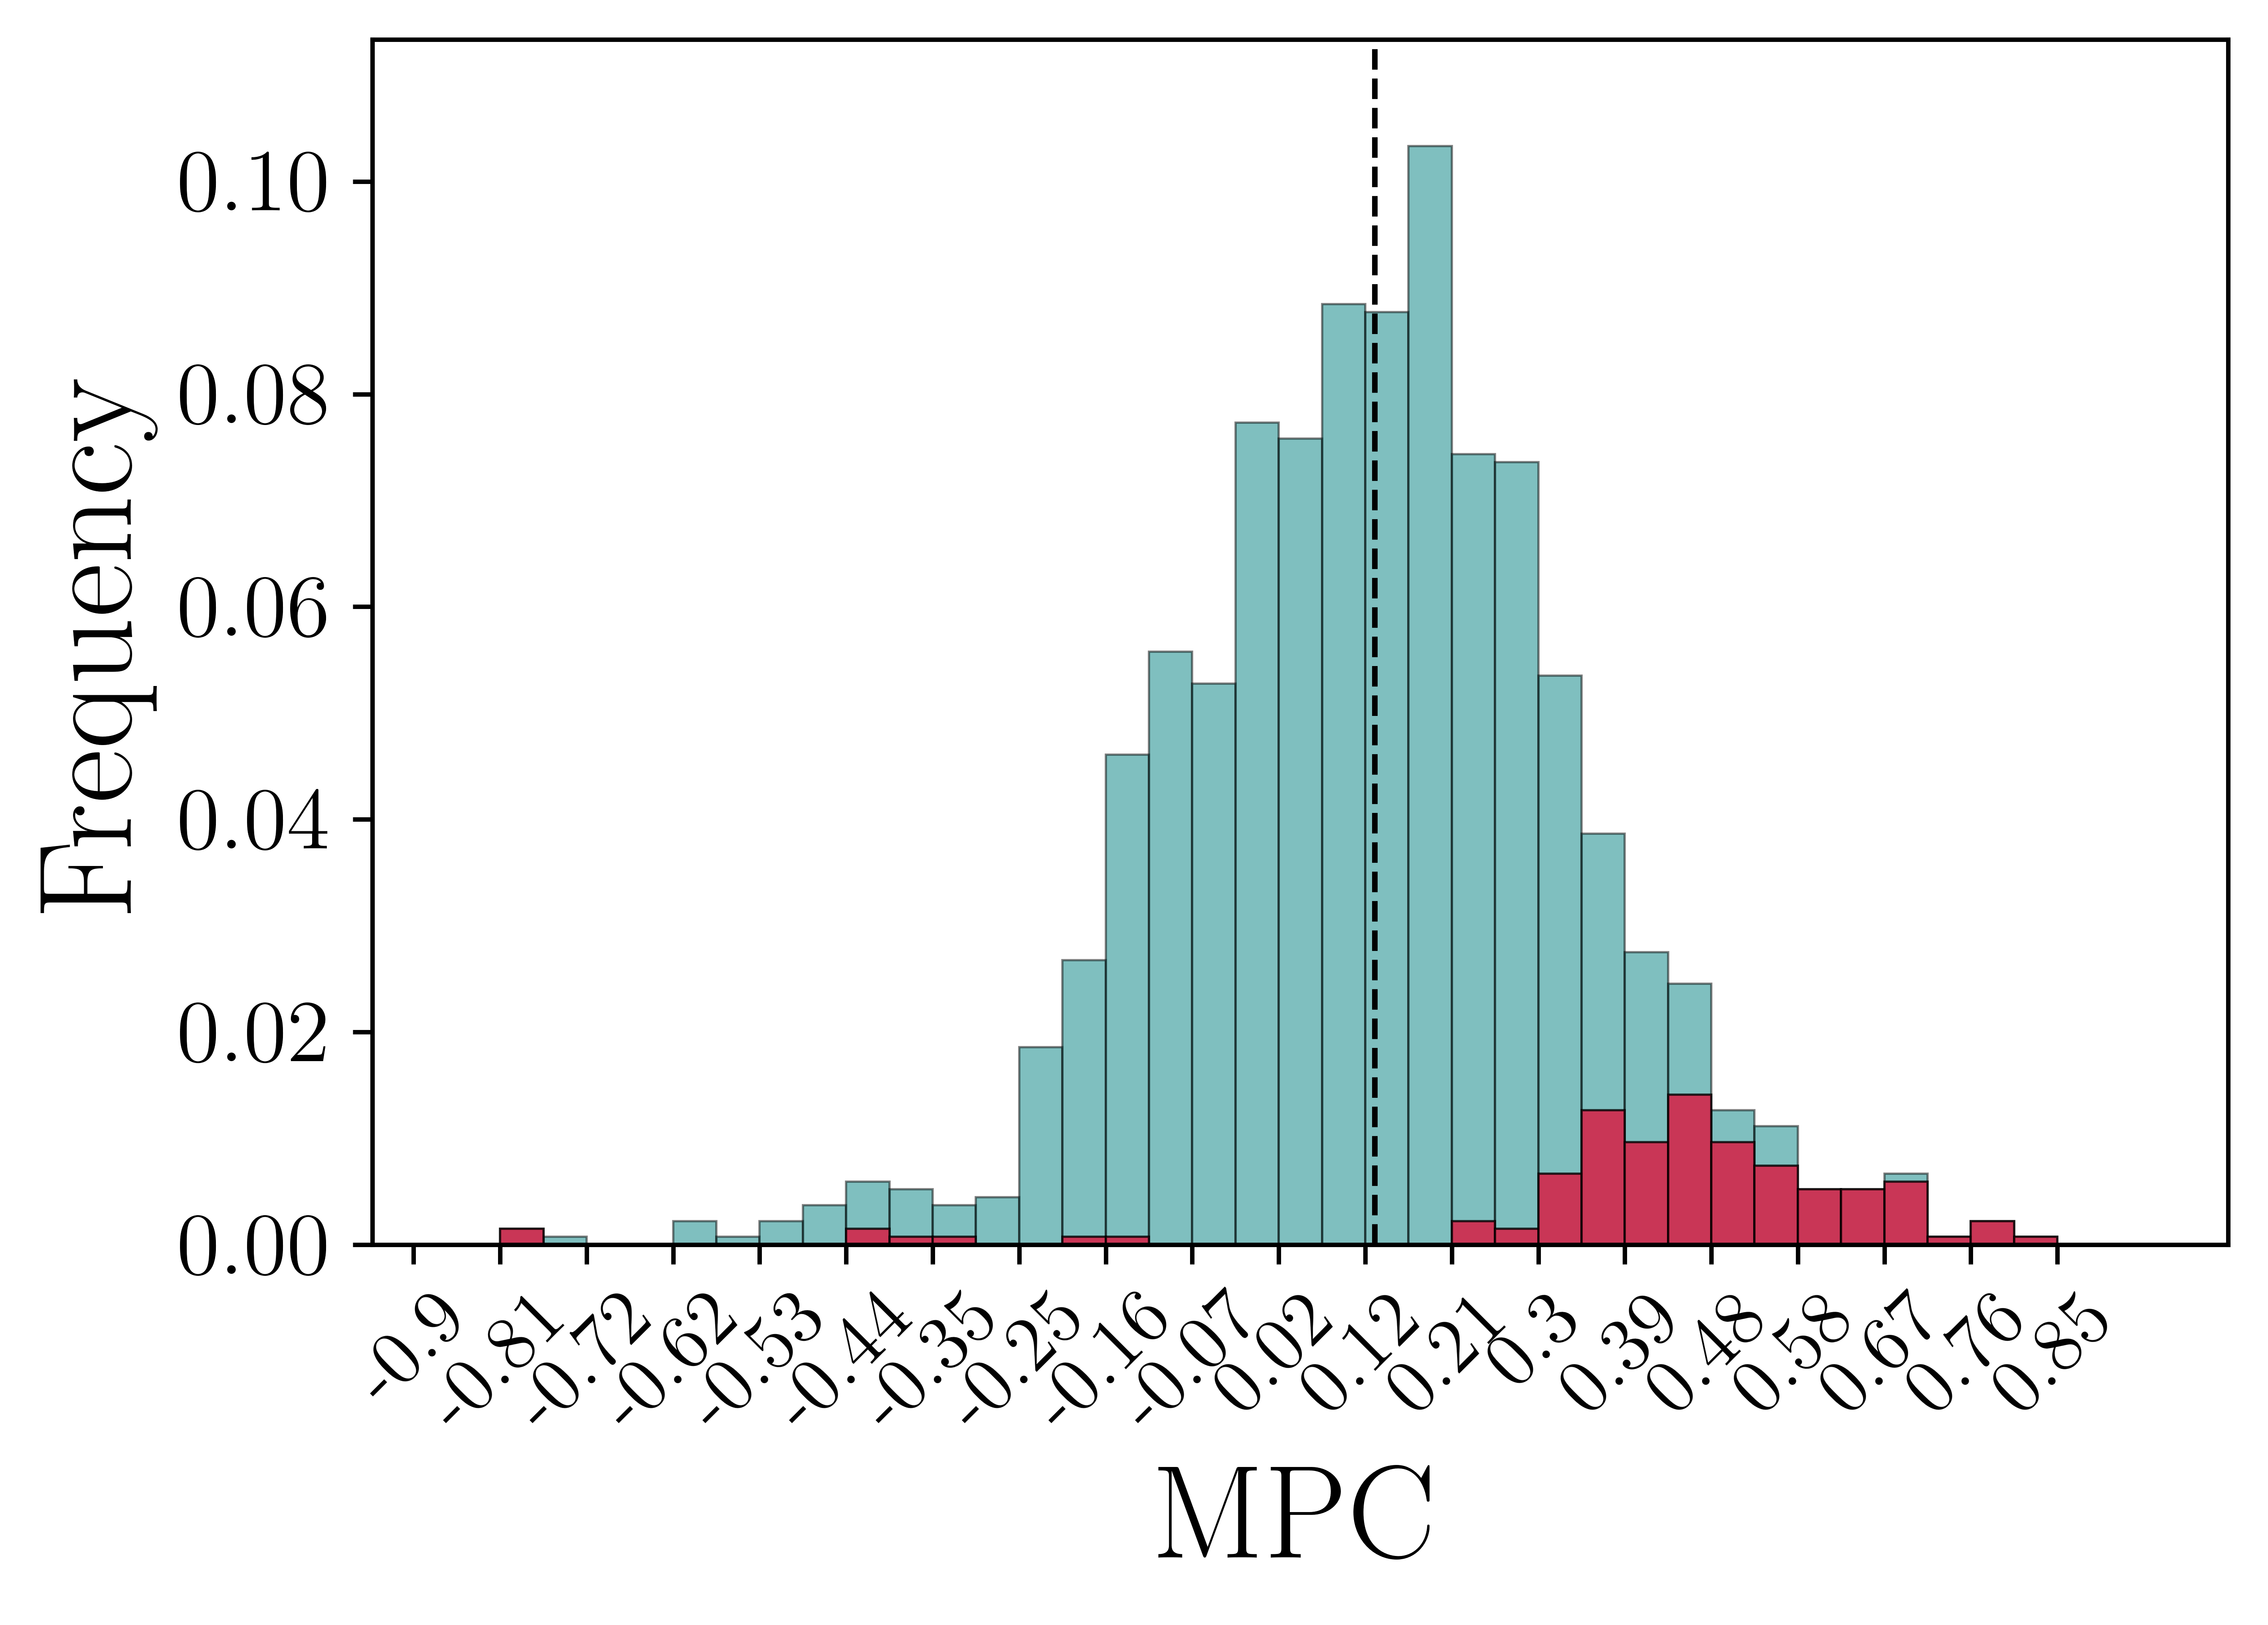
\includegraphics[width=\linewidth]{figures/distributions/spec3_cf_chNDexp.png}
        \caption{Spec 3 - causal forest}
    \end{subfigure}\hfill
    \fnote{Blue parts show frequency of point estimates in this bin, red parts show share of these being statistically significant with $p\leq0.1$. Dotted lines signal the \textit{Average Treatment Effect}.}
    \caption{Distributions of estimated MPC - non-durable expenditures}
    \label{fig:dist_nd}
\end{figure}
\begin{figure}[t]
    \centering
%    \mbox{}\hfill
    \begin{subfigure}{0.33\linewidth}
        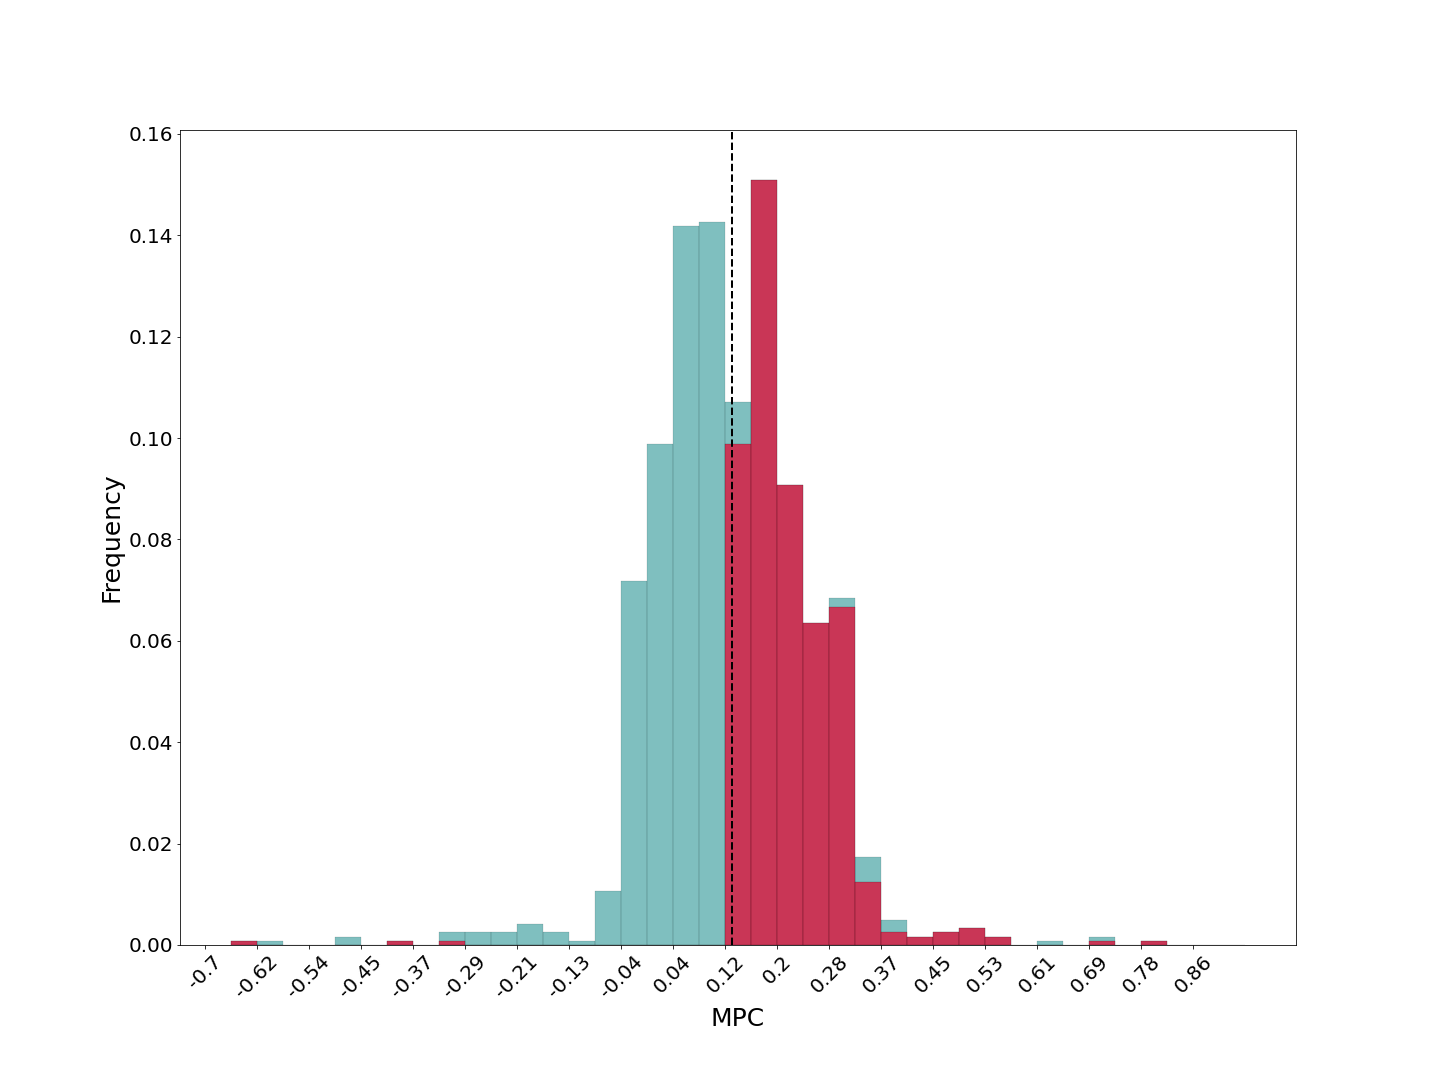
\includegraphics[width=\linewidth]{figures/distributions/spec1_lin_chSNDexp.png}
        \caption{Spec 1 - linear}
    \end{subfigure}\hfill
    \begin{subfigure}{0.33\linewidth}
        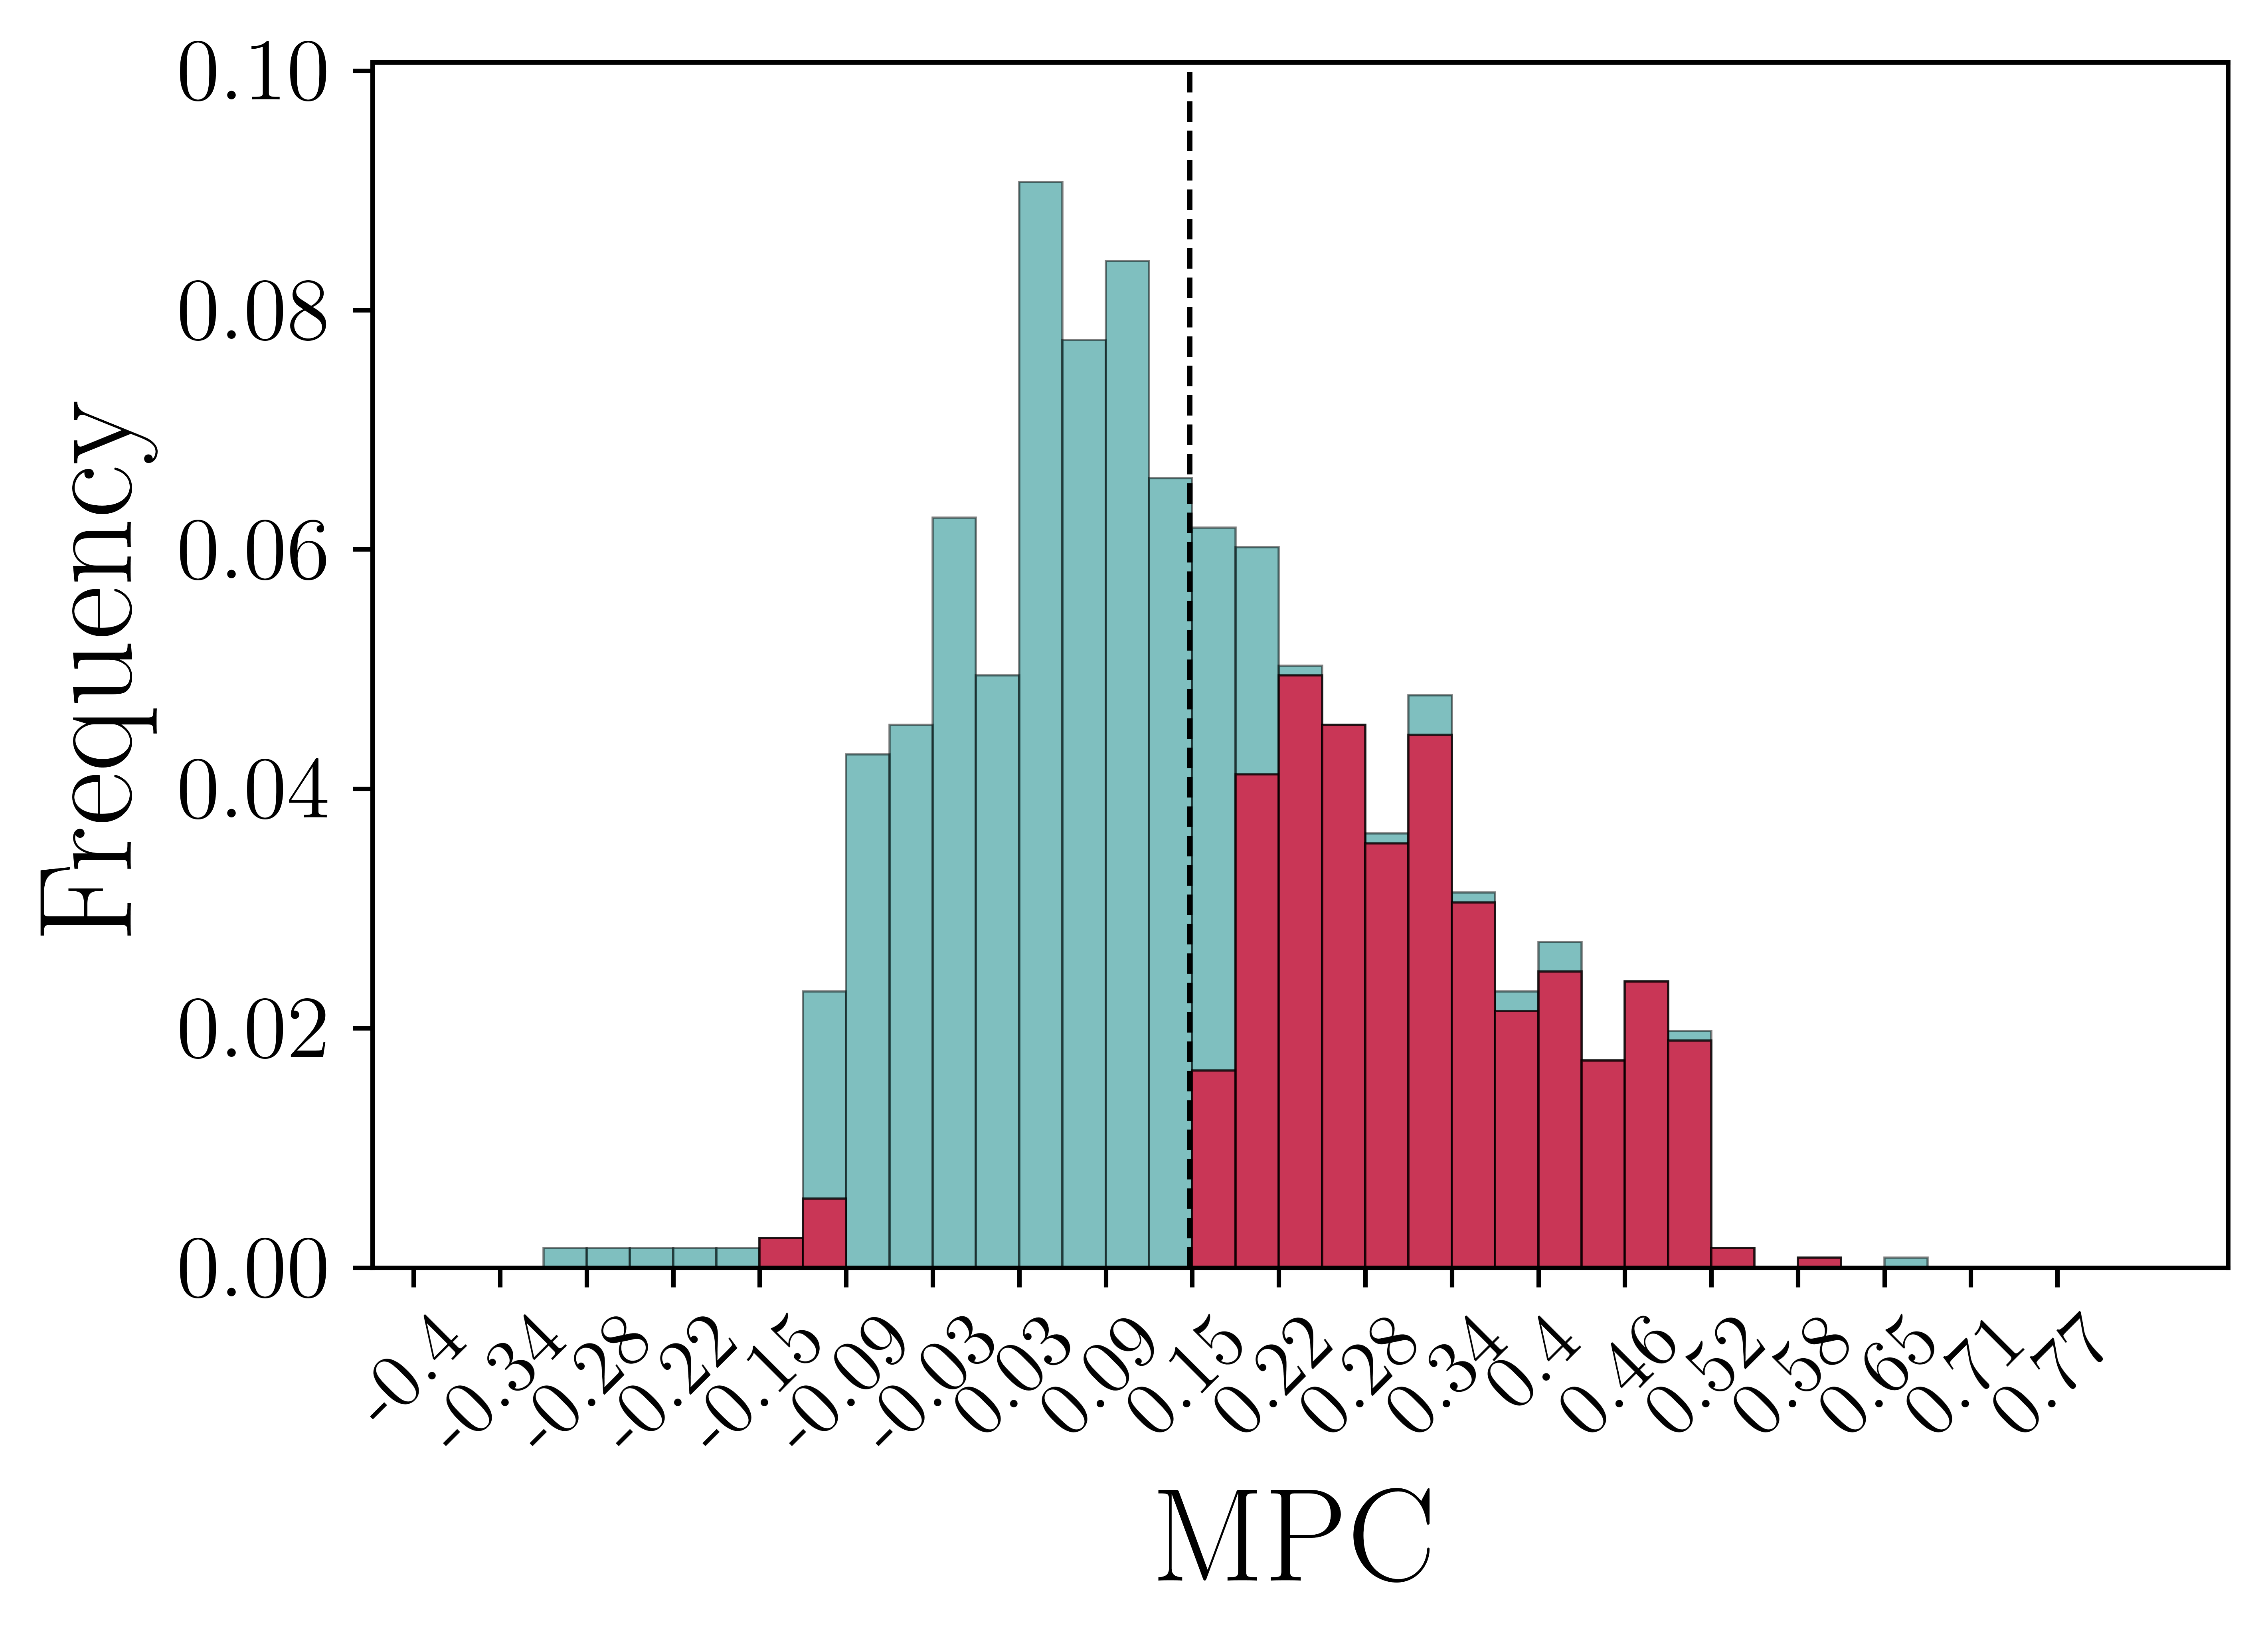
\includegraphics[width=\linewidth]{figures/distributions/spec2_lin_chSNDexp.png}
        \caption{Spec 2 - linear}
    \end{subfigure}\hfill
    \begin{subfigure}{0.33\linewidth}
        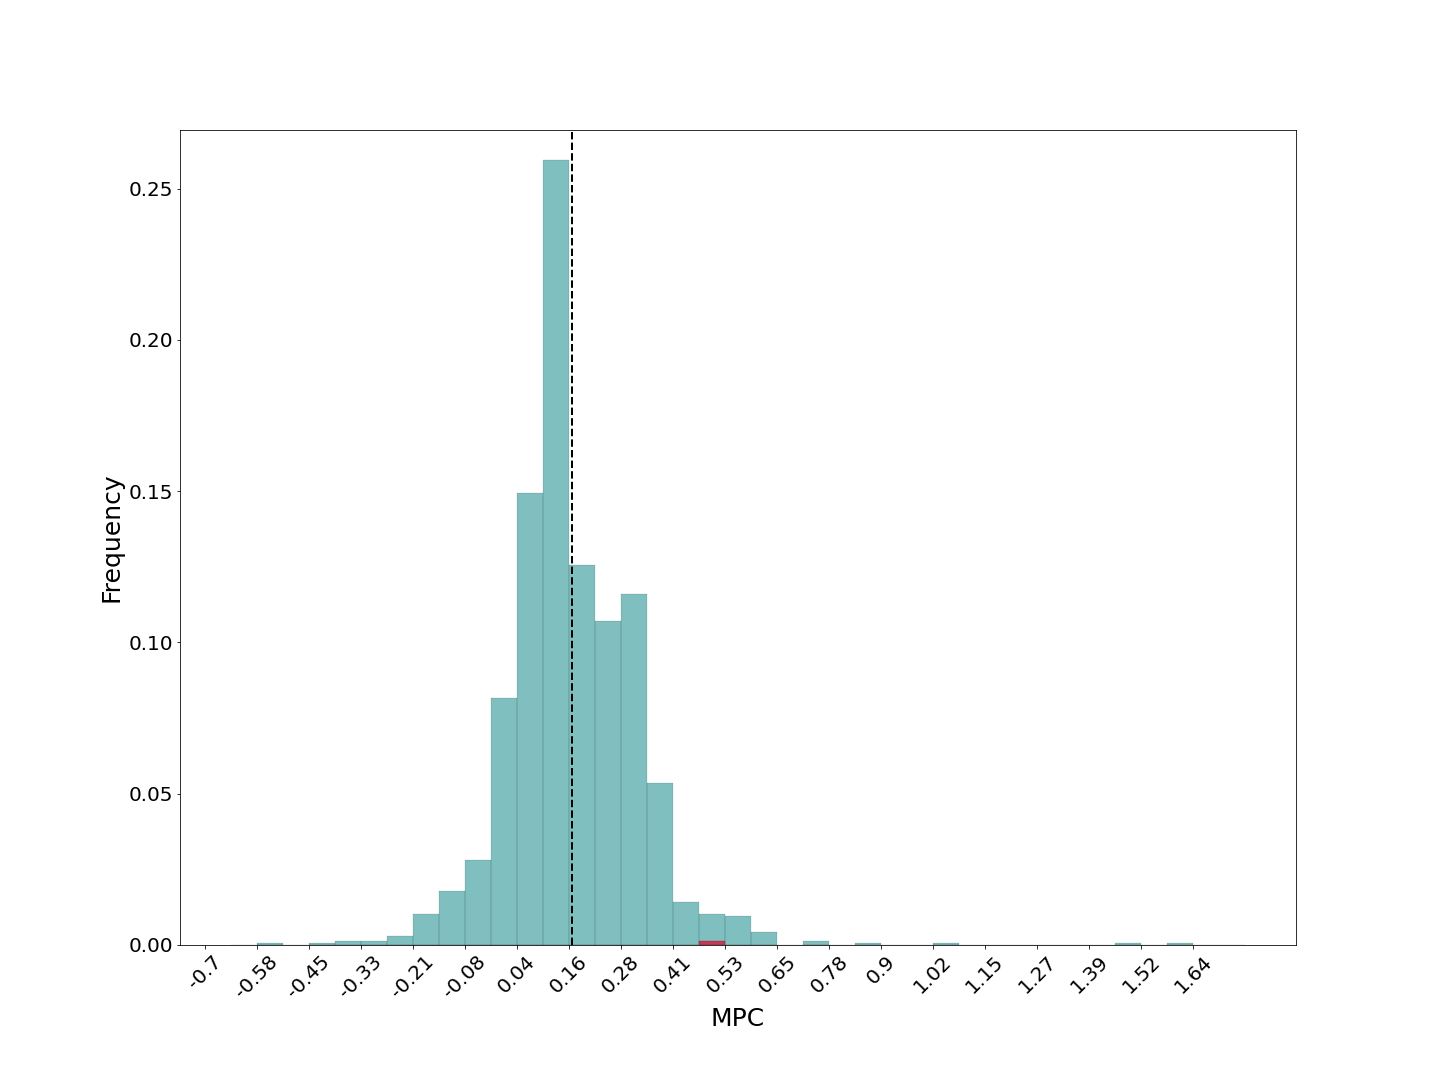
\includegraphics[width=\linewidth]{figures/distributions/spec3_lin_chSNDexp.png}
        \caption{Spec 3 - linear}
    \end{subfigure}\hfill
    
%    \mbox{}\hfill
    \begin{subfigure}{0.33\linewidth}
        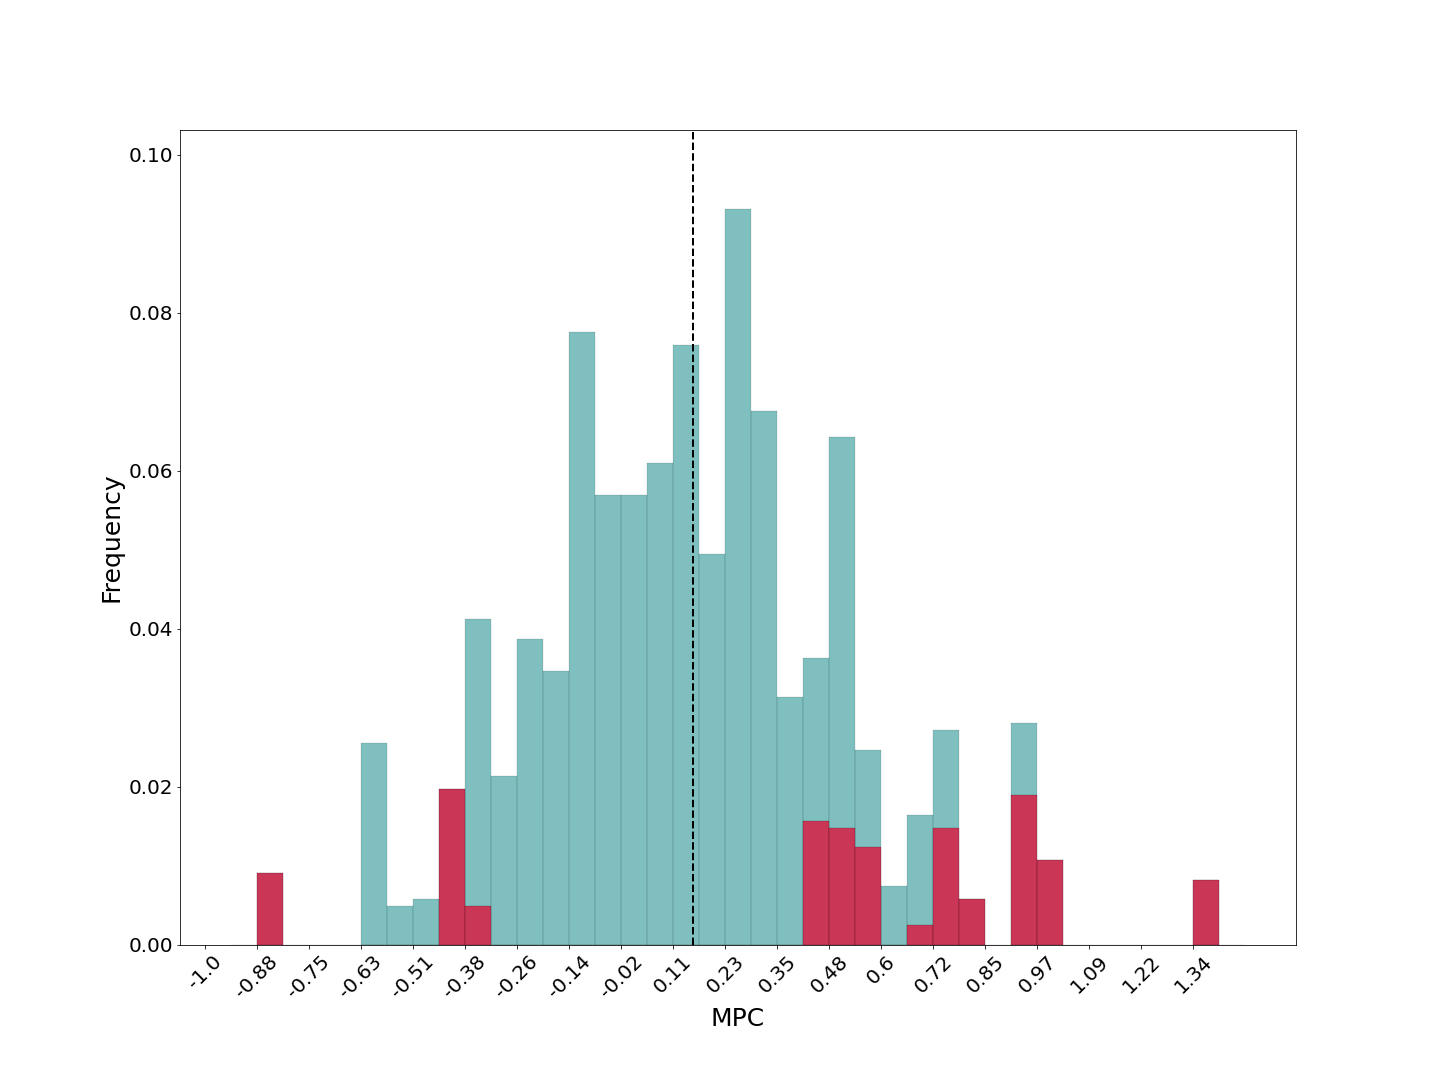
\includegraphics[width=\linewidth]{figures/distributions/spec1_cf_chSNDexp.png}
        \caption{Spec 1 - causal forest}
    \end{subfigure}\hfill
    \begin{subfigure}{0.33\linewidth}
        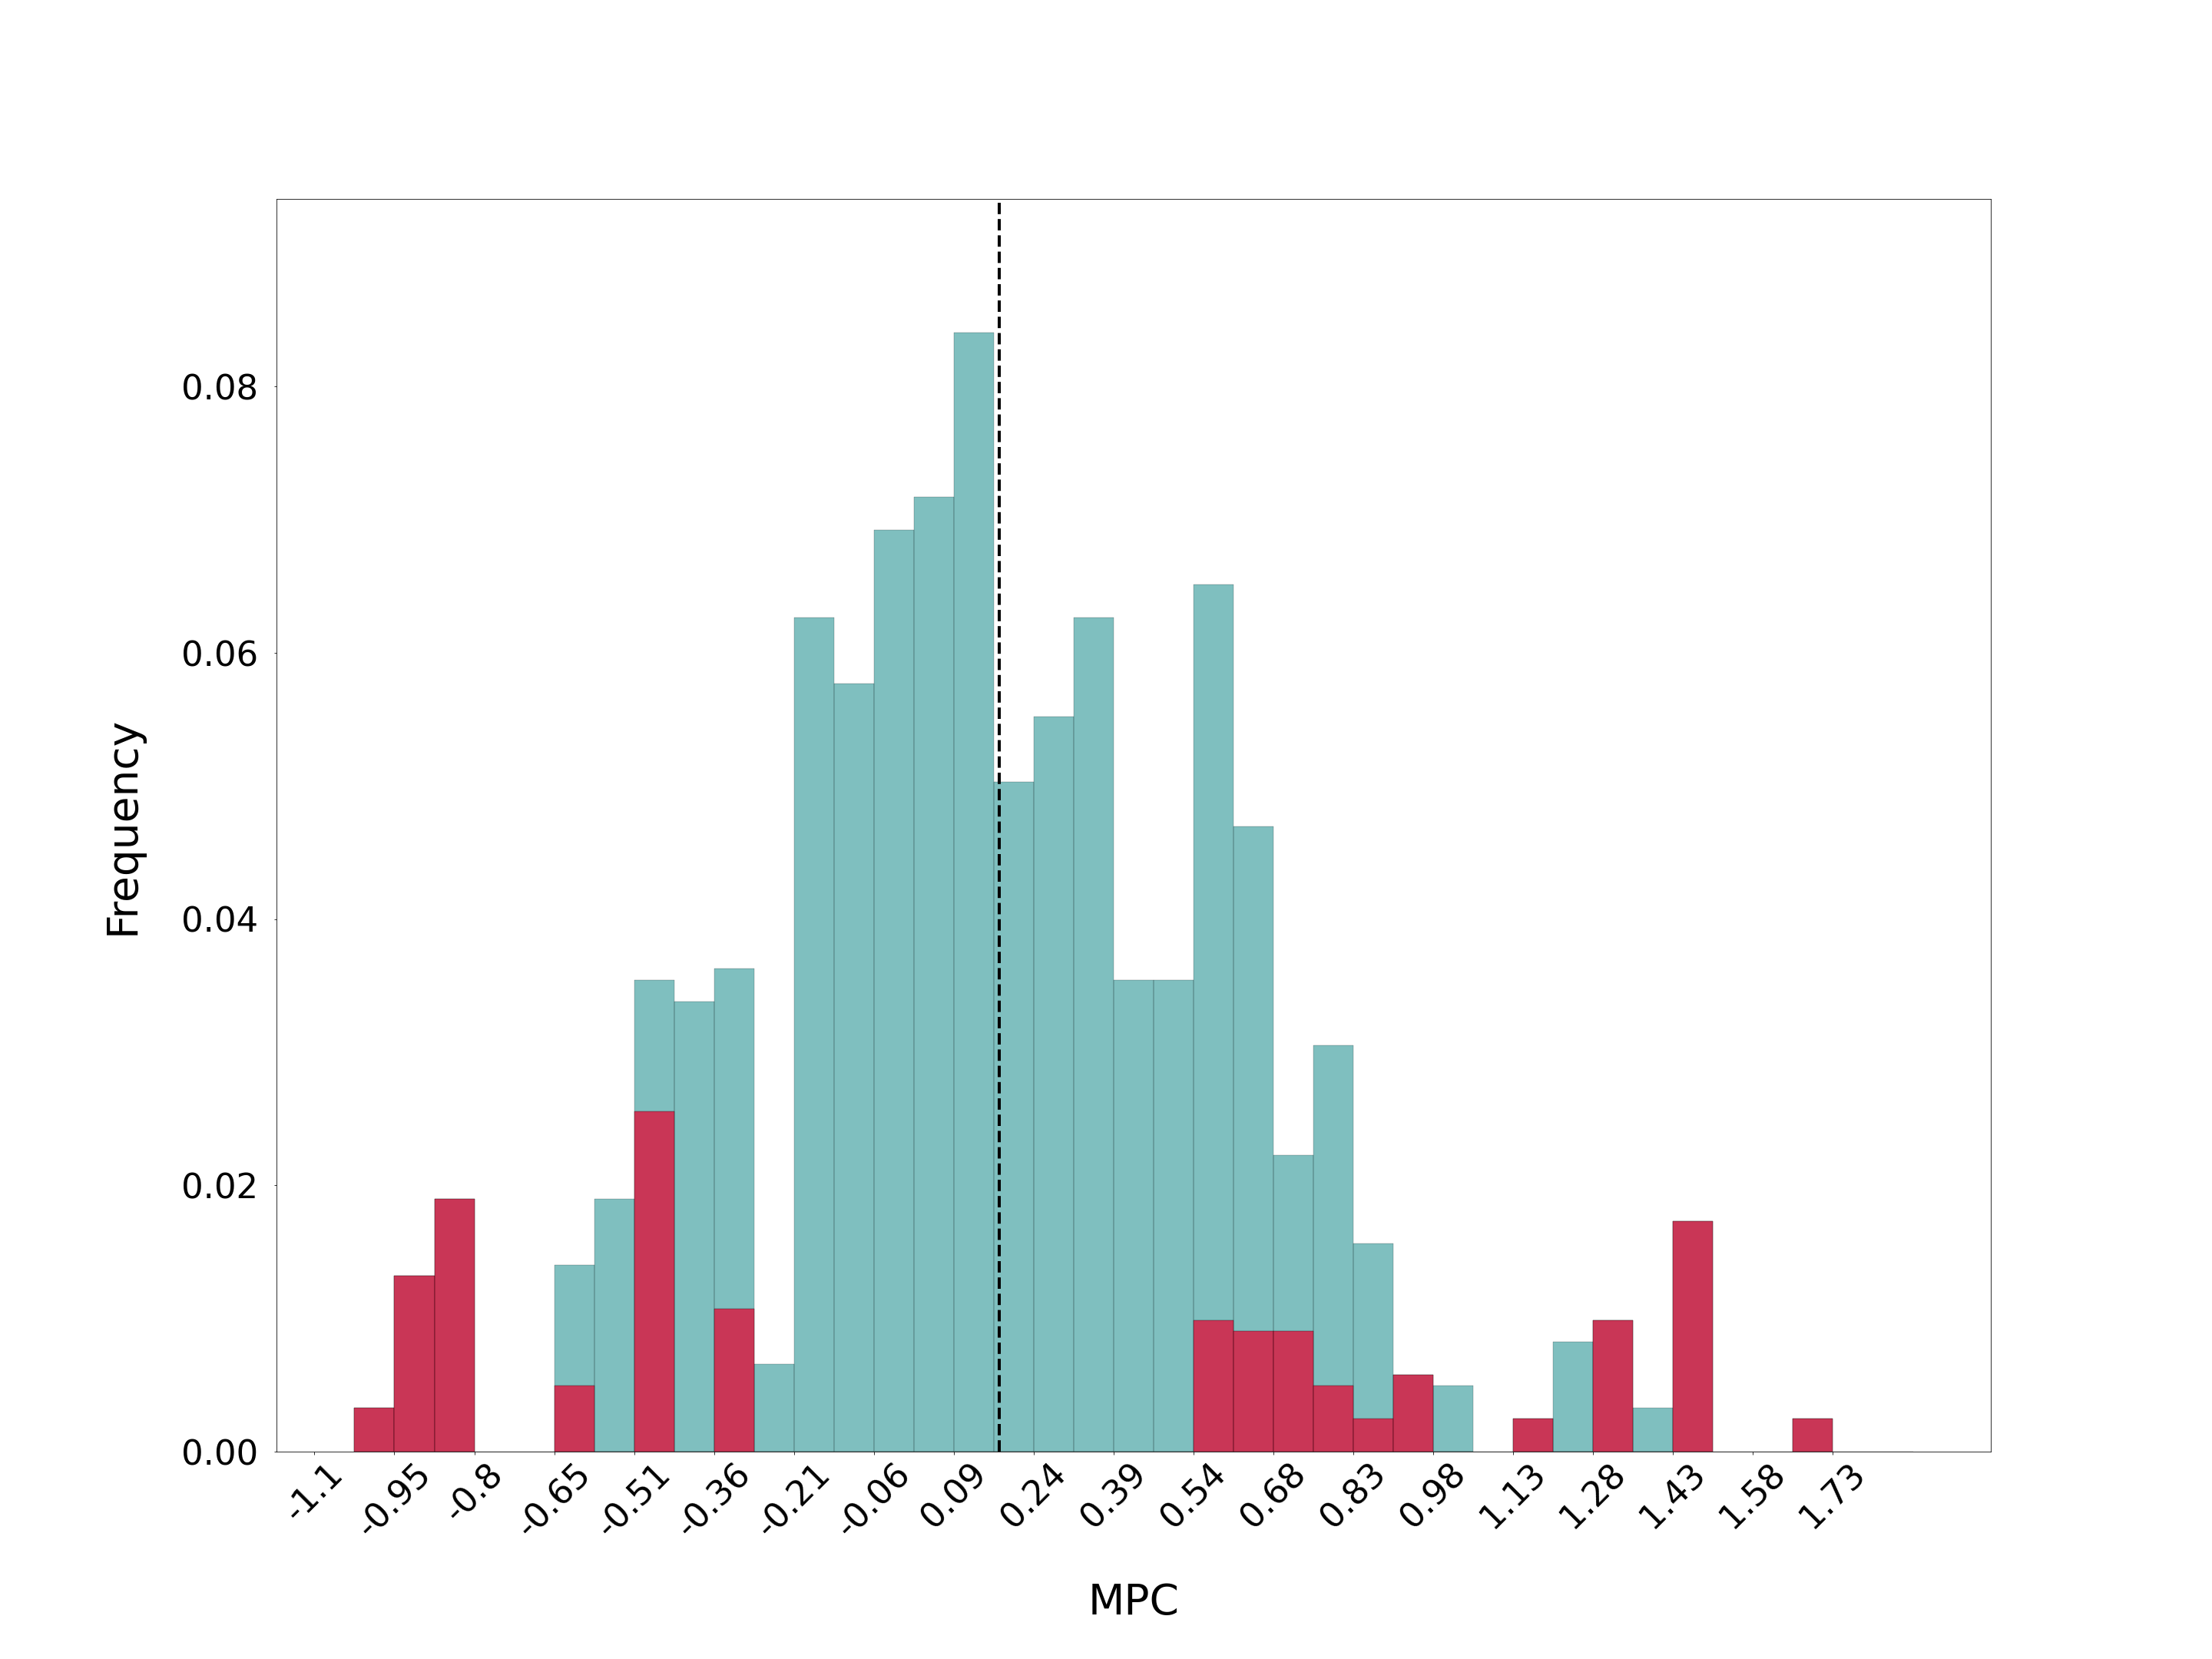
\includegraphics[width=\linewidth]{figures/distributions/spec2_cf_chSNDexp.png}
        \caption{Spec 2 - causal forest}
    \end{subfigure}\hfill
    \begin{subfigure}{0.33\linewidth}
        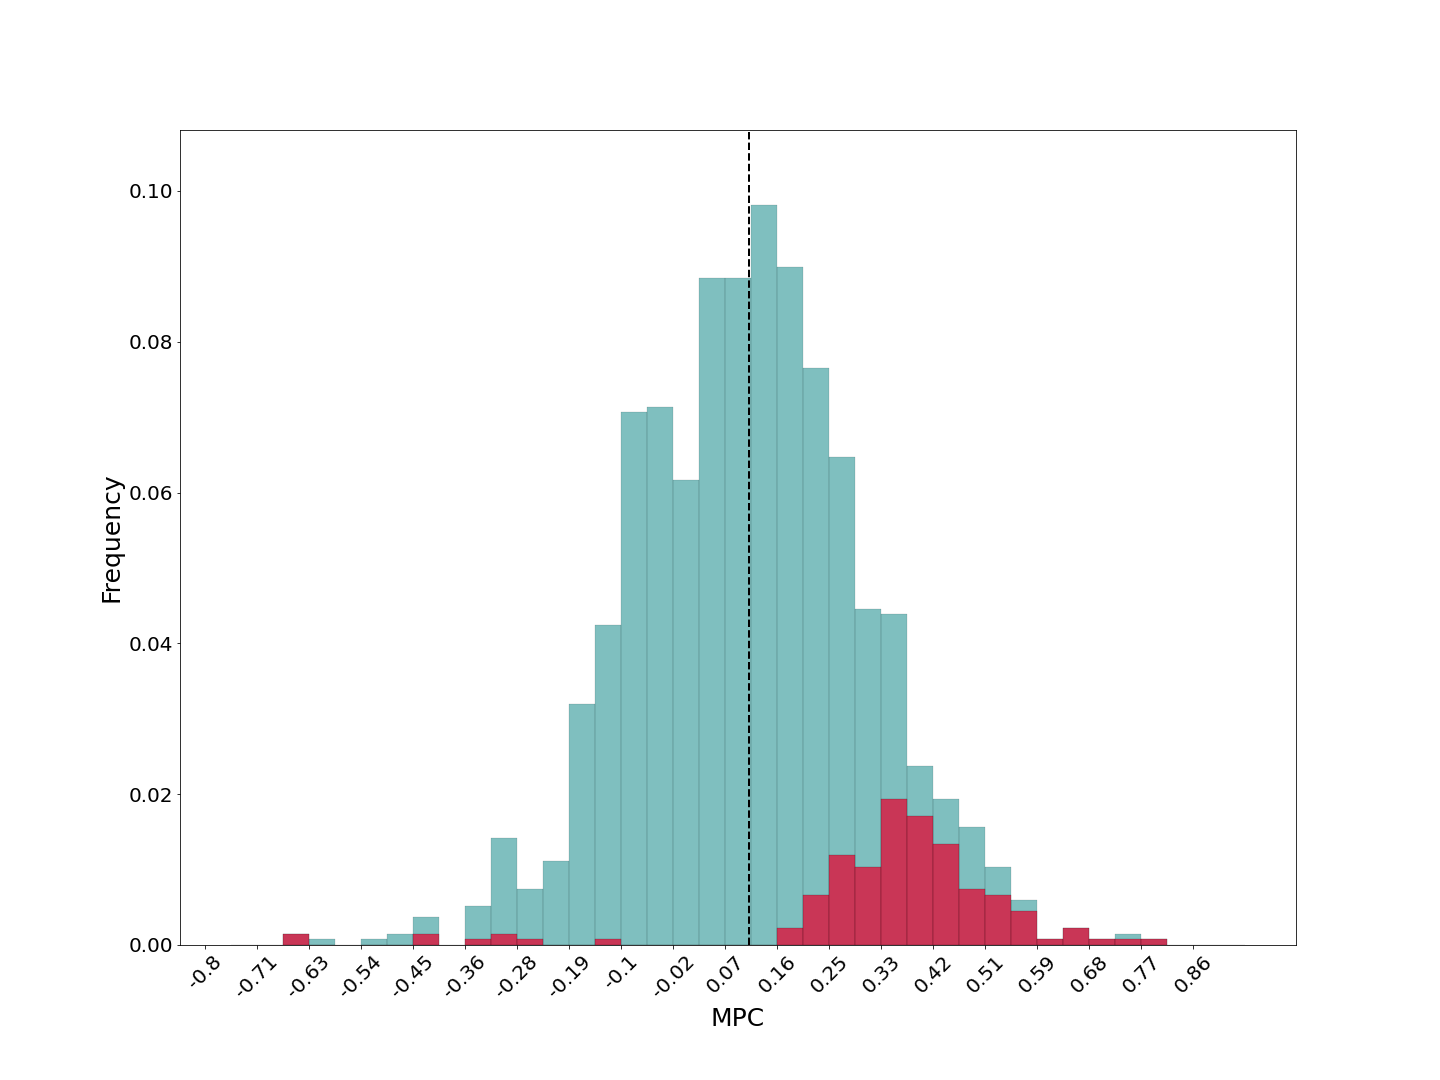
\includegraphics[width=\linewidth]{figures/distributions/spec3_cf_chSNDexp.png}
        \caption{Spec 3 - causal forest}
    \end{subfigure}\hfill
    \fnote{Blue parts show frequency of point estimates in this bin, red parts show share of these being statistically significant with $p\leq0.1$. Dotted lines signal the \textit{Average Treatment Effect}.}
    \caption{Distributions of estimated MPC - strictly non-durable expenditures}
    \label{fig:dist_snd}
\end{figure}
\begin{figure}[t]
    \centering
%    \mbox{}\hfill
    \begin{subfigure}{0.33\linewidth}
        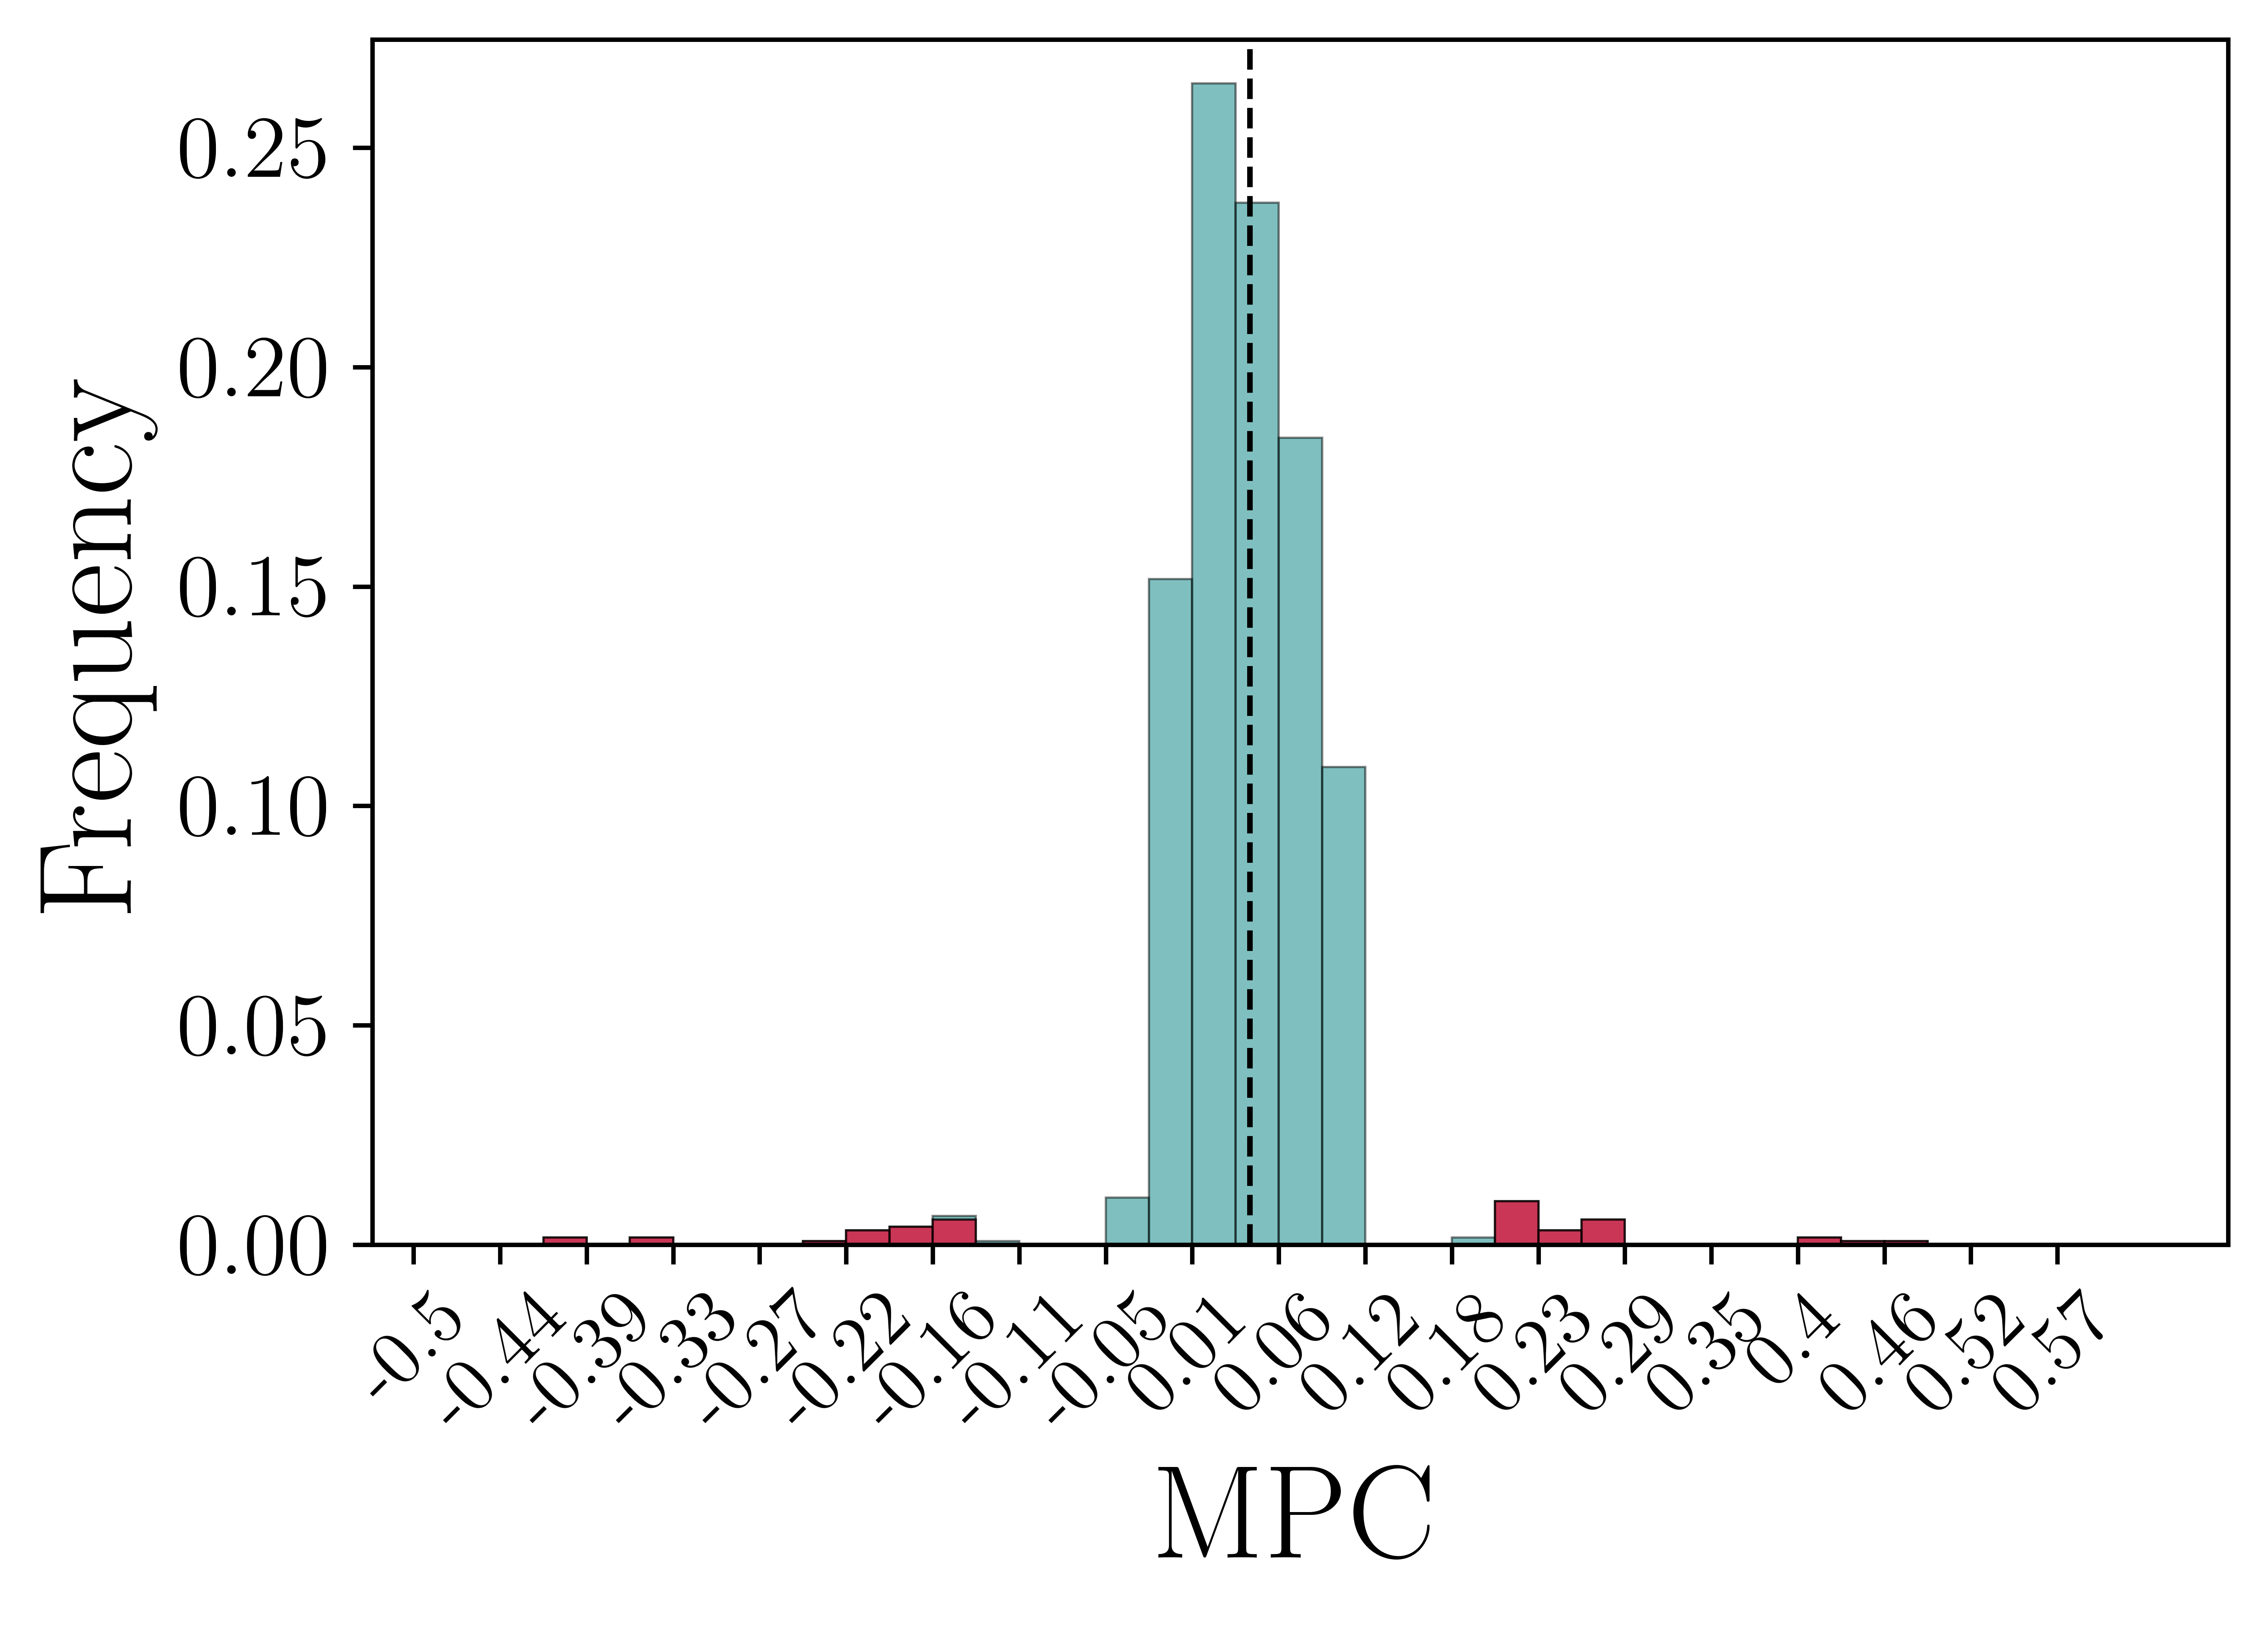
\includegraphics[width=\linewidth]{figures/distributions/spec1_lin_chFDexp.png}
        \caption{Spec 1 - linear}
    \end{subfigure}\hfill
    \begin{subfigure}{0.33\linewidth}
        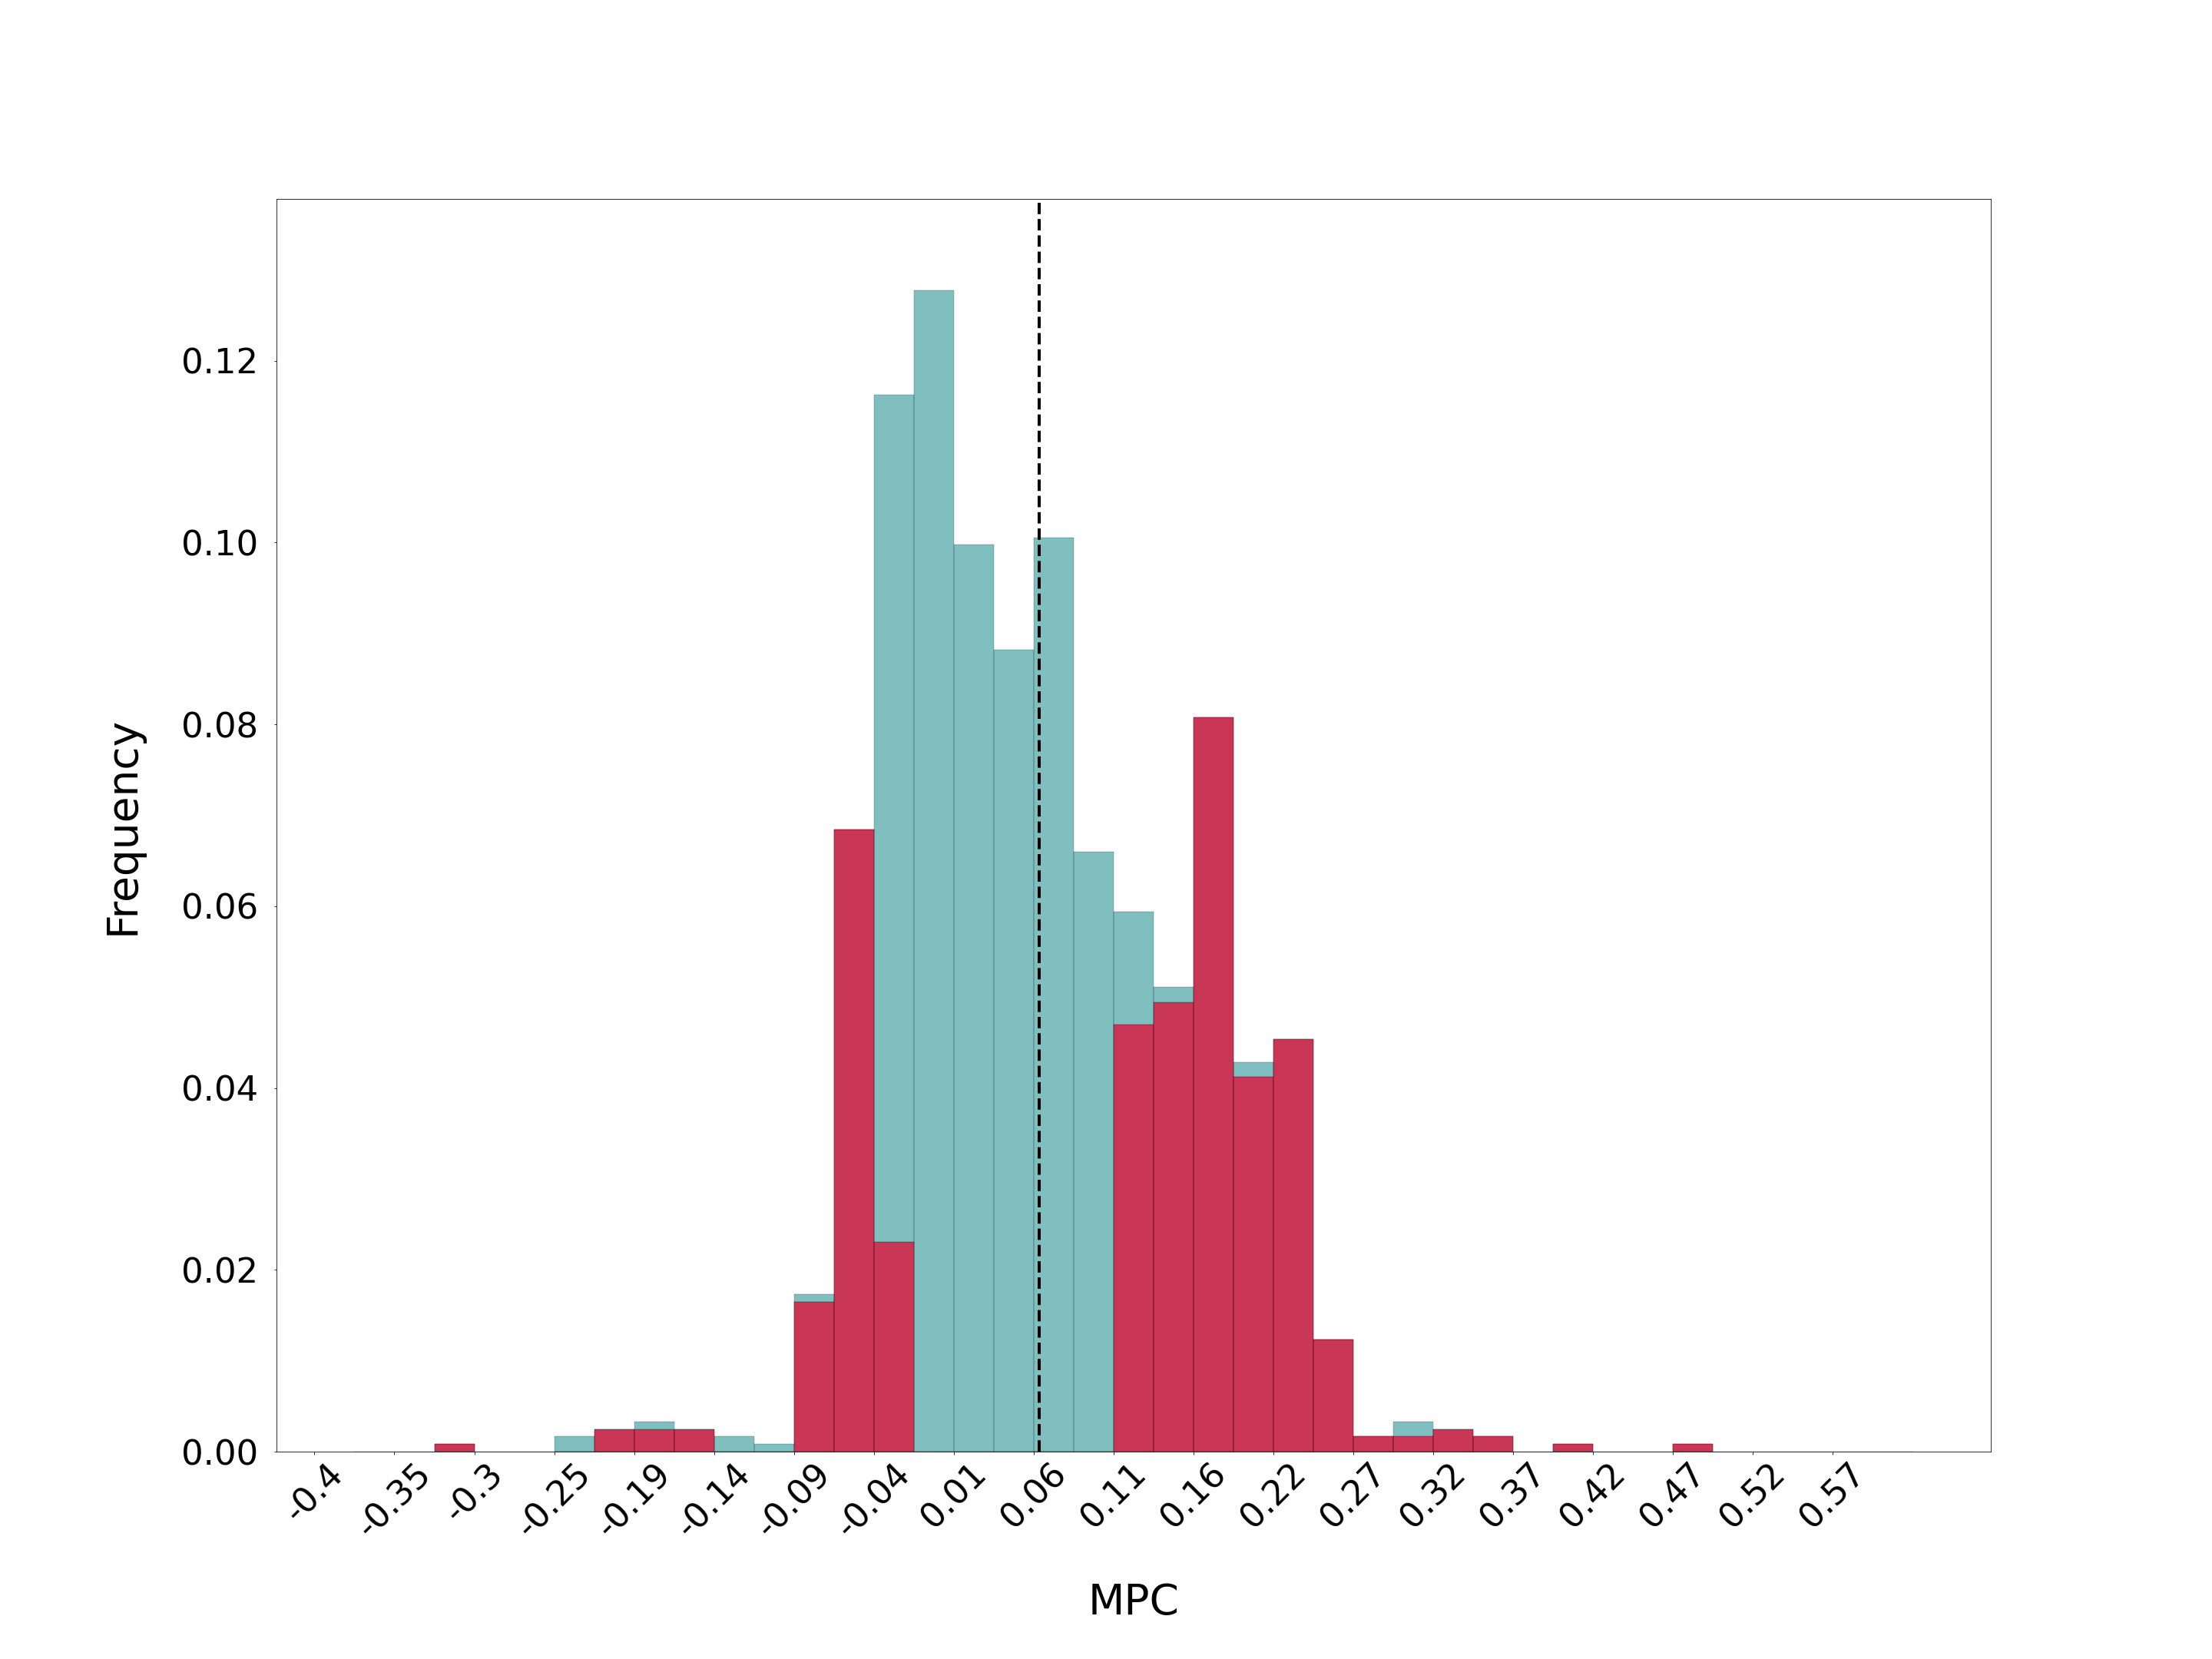
\includegraphics[width=\linewidth]{figures/distributions/spec2_lin_chFDexp.png}
        \caption{Spec 2 - linear}
    \end{subfigure}\hfill
    \begin{subfigure}{0.33\linewidth}
        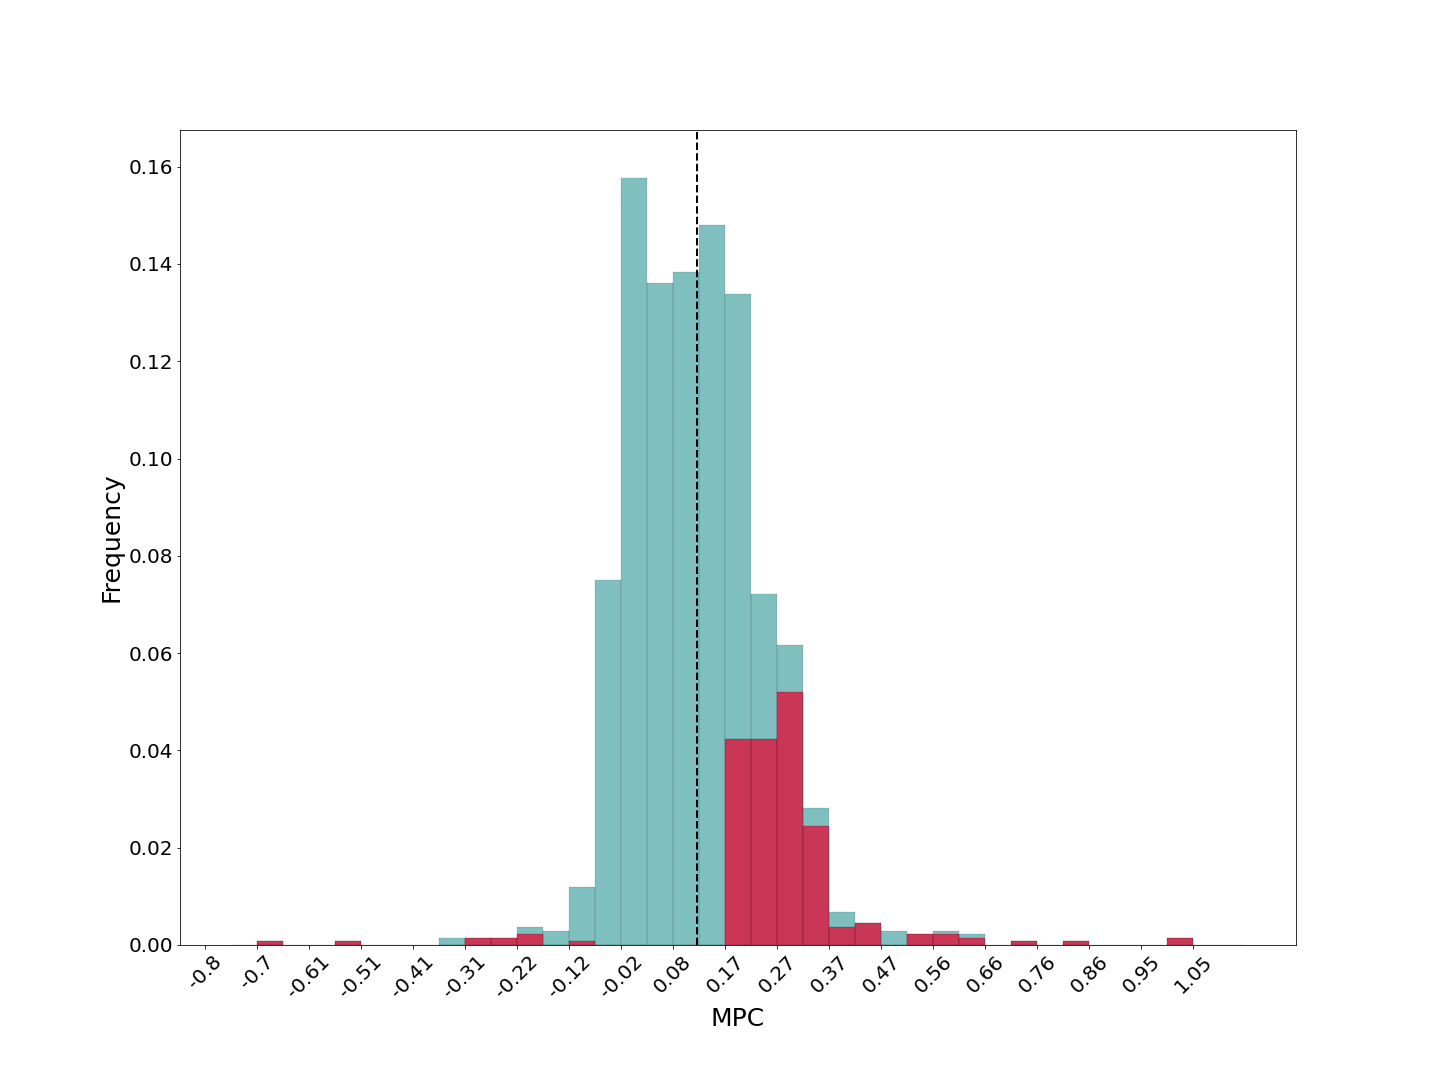
\includegraphics[width=\linewidth]{figures/distributions/spec3_lin_chFDexp.png}
        \caption{Spec 3 - linear}
    \end{subfigure}\hfill
    
%    \mbox{}\hfill
    \begin{subfigure}{0.33\linewidth}
        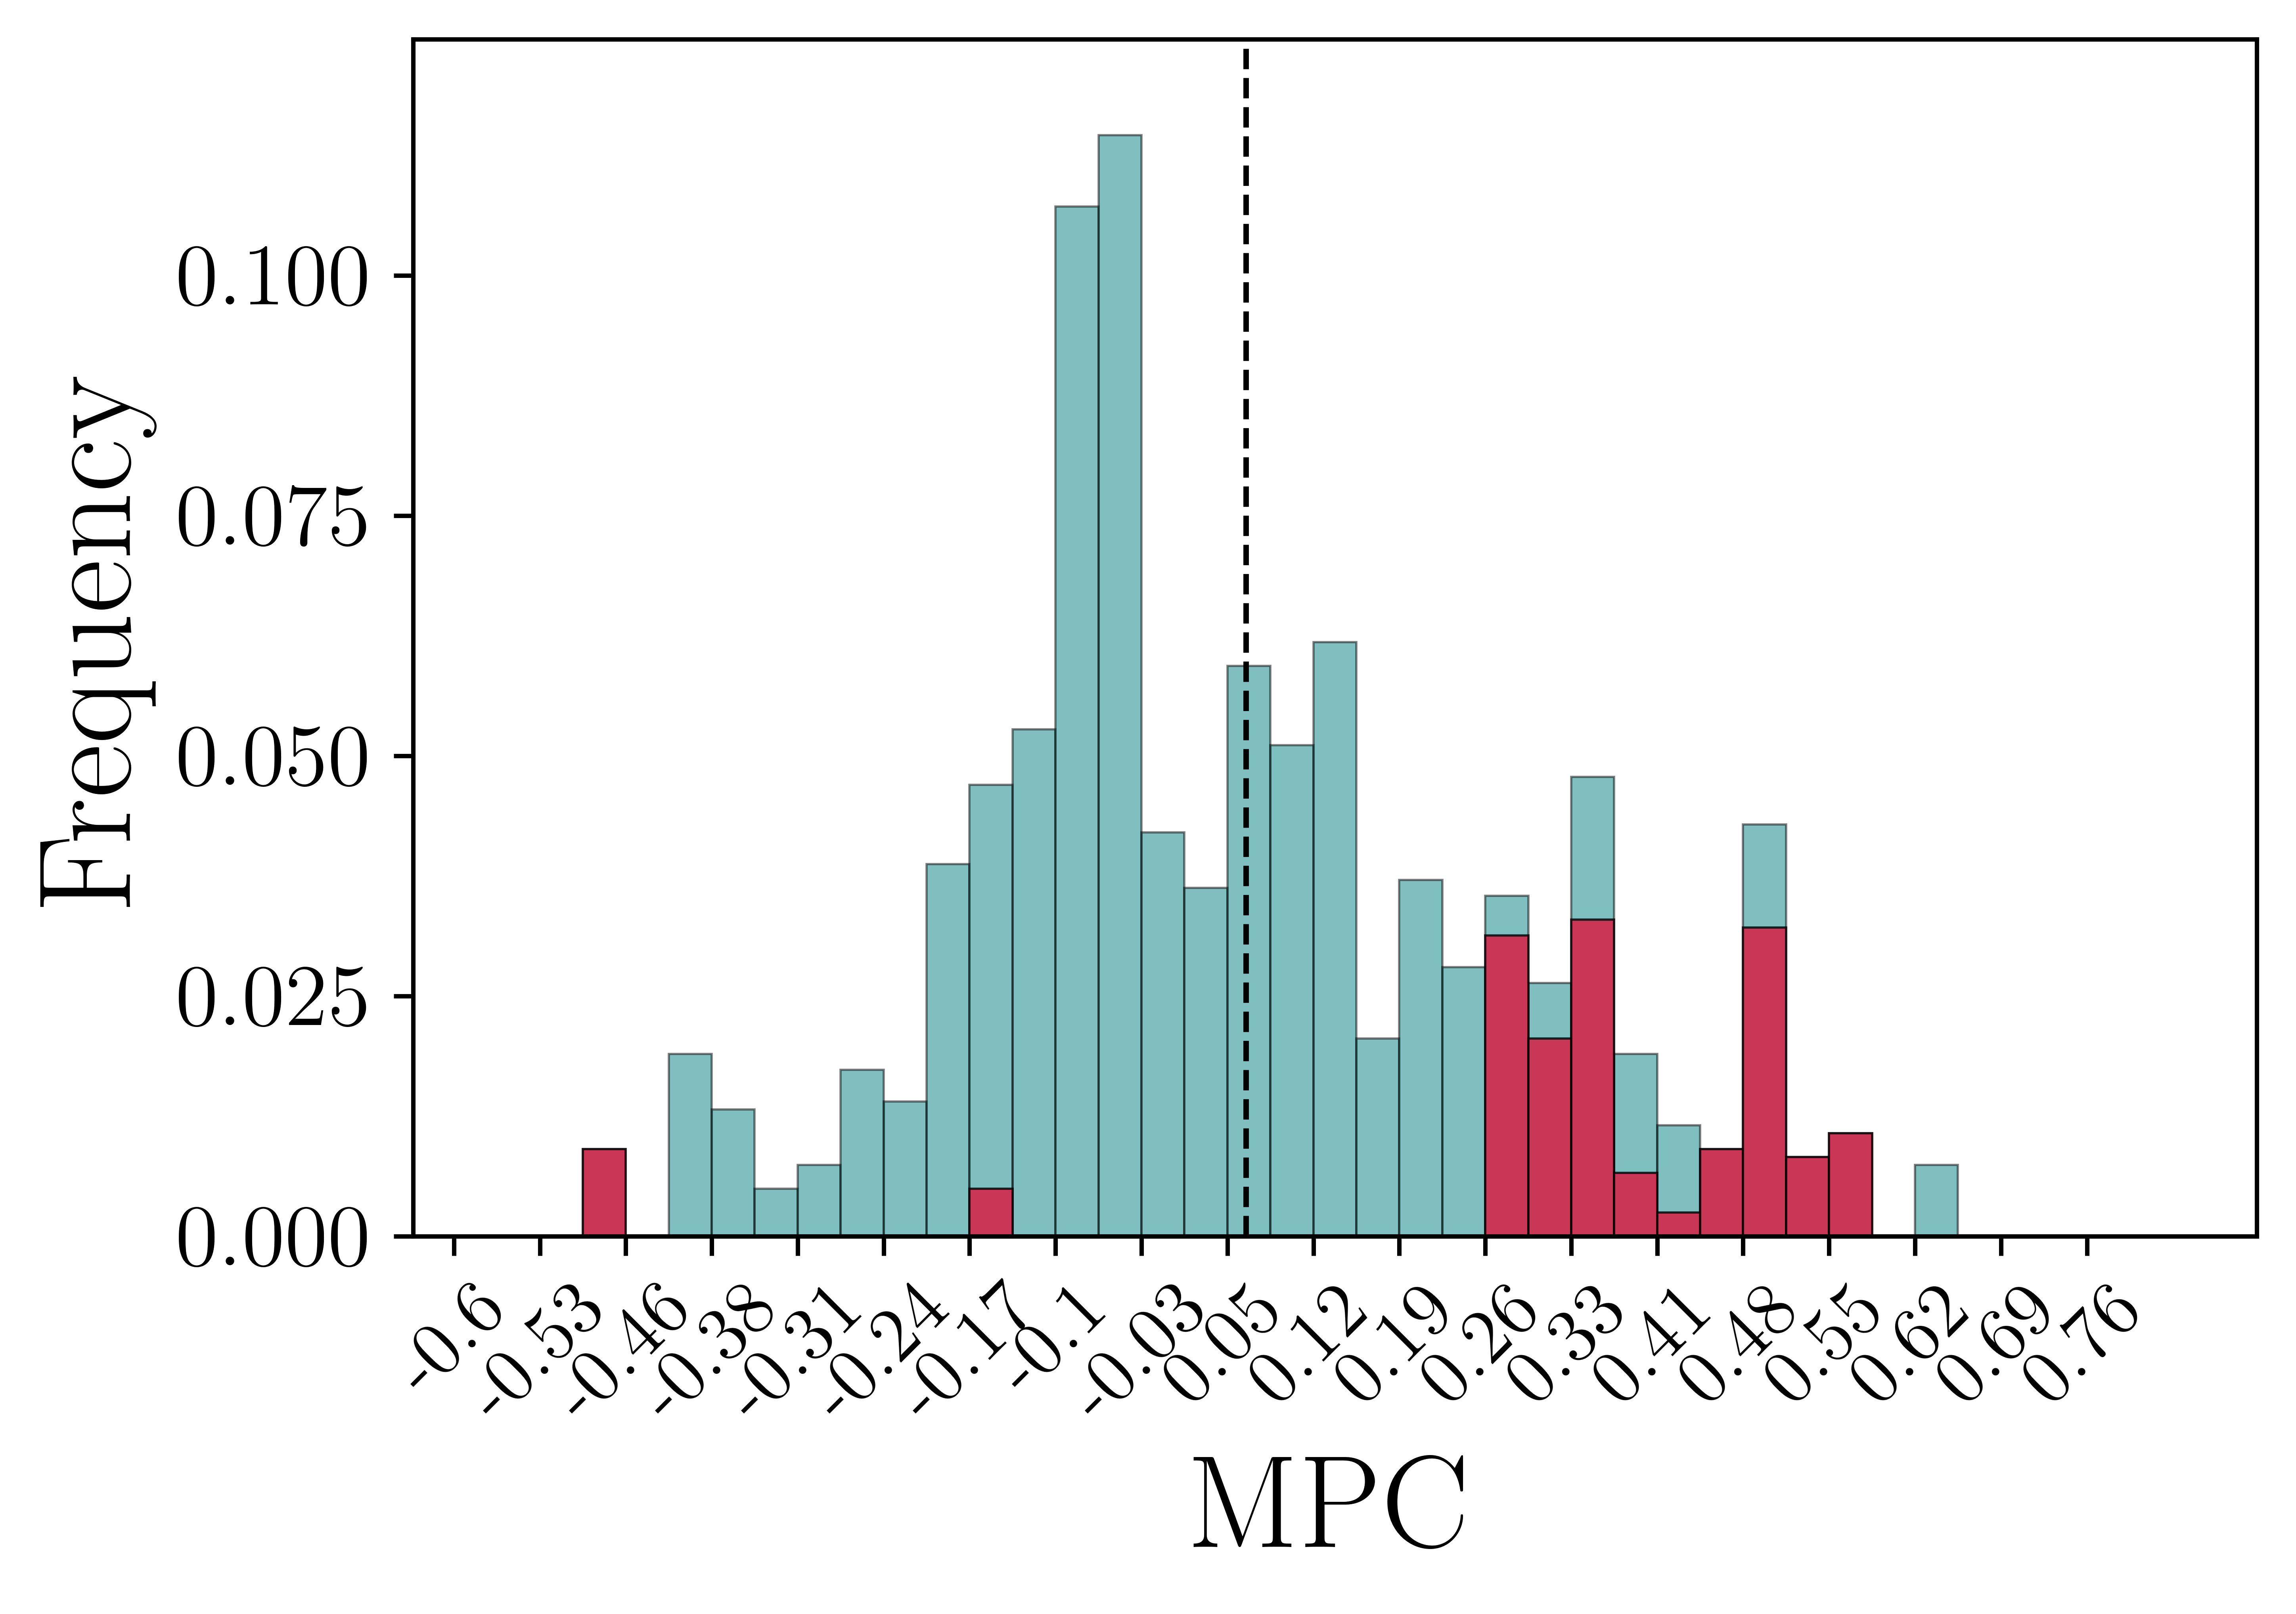
\includegraphics[width=\linewidth]{figures/distributions/spec1_cf_chFDexp.png}
        \caption{Spec 1 - causal forest}
    \end{subfigure}\hfill
    \begin{subfigure}{0.33\linewidth}
        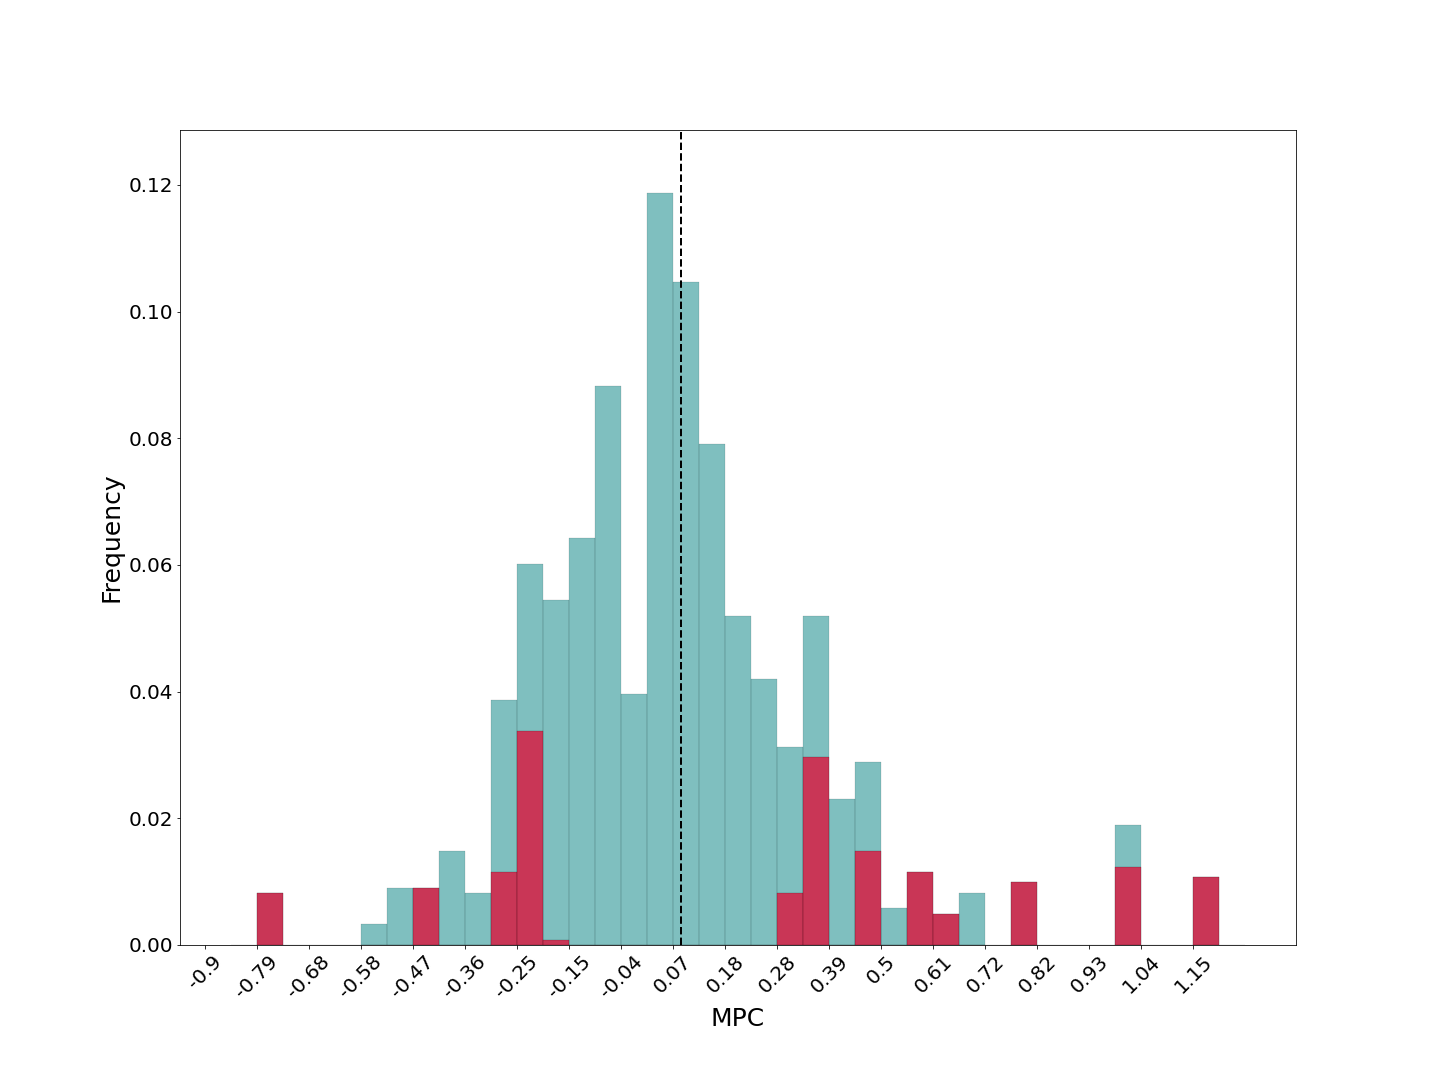
\includegraphics[width=\linewidth]{figures/distributions/spec2_cf_chFDexp.png}
        \caption{Spec 2 - causal forest}
    \end{subfigure}\hfill
    \begin{subfigure}{0.33\linewidth}
        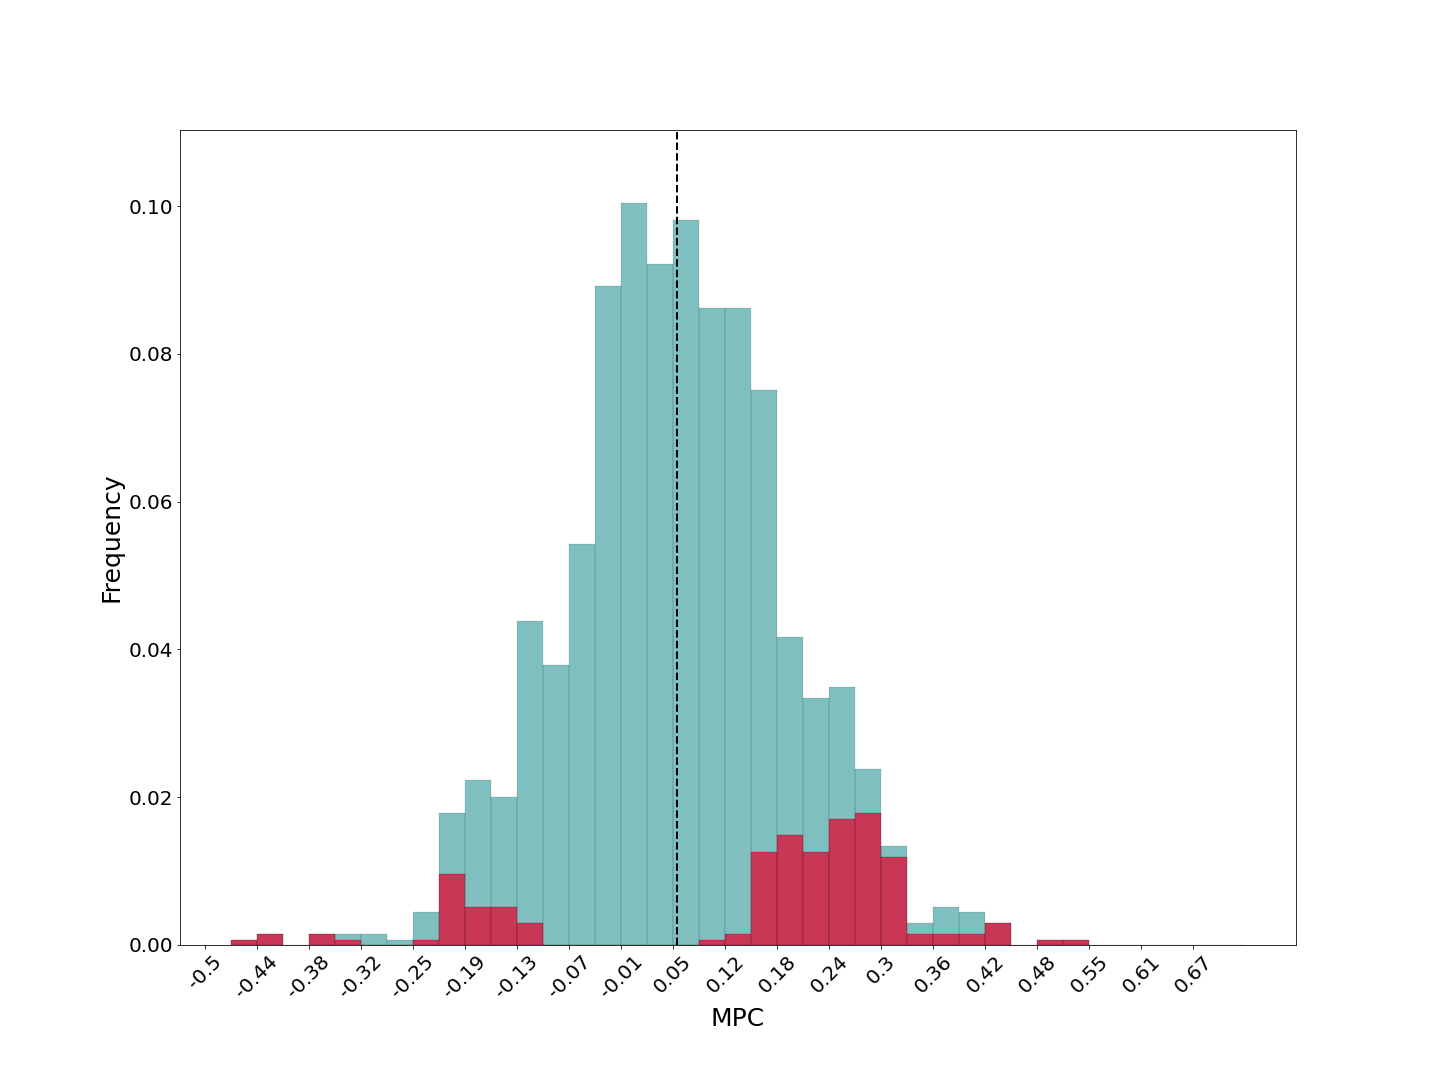
\includegraphics[width=\linewidth]{figures/distributions/spec3_cf_chFDexp.png}
        \caption{Spec 3 - causal forest}
    \end{subfigure}\hfill
    \fnote{Blue parts show frequency of point estimates in this bin, red parts show share of these being statistically significant with $p\leq0.1$. Dotted lines signal the \textit{Average Treatment Effect}.}
    \caption{Distributions of estimated MPC - food expenditures}
    \label{fig:dist_fd}
\end{figure}
\noindent In general, we find strong support for heterogeneity in the Marginal Propensity to Consume. The plots in Figures \ref{fig:dist_tot} to \ref{fig:dist_fd} show a large variation of MPCs across all consumption categories and estimation approaches. This underlines the importance of accounting for heterogeneous responses to income shocks. The heterogeneity is similar to Misra and Surico’s findings. Our results show a large mass of households having a Marginal Propensity to Consume close to 0 and for many households, we cannot reject the null hypothesis of a zero MPC. On the other hand, there is a smaller share of households that show strong, significant responses. Table \ref{tab:sig_shares} depicts the shares of significant MPCs we estimate for each specification and model when we look at changes in non-durable consumption.\footnote{Significance shares for the other three main outcomes discussed in this section are reported in Appendix \ref{app:sig_shares}.} \\
Meanwhile, the ATE is very close to zero in all expenditure categories (except TOT) and across all estimations the bin it falls into never contains more than 15\% of all point estimates. This highlights the weak representativeness of the ATE and its inability to reliably assess the success of programs such as the 2008 tax stimulus. Accounting for heterogeneity reveals positive effects of the stimulus program on household spending that far exceed the average responses. \\
Taking a look at the measure of interest, the conditional average treatment effect, the similarity of our results to Misra and Surico's depends on our specification and choice of estimator. Using the linear DML, we find similar results across all expenditure categories in specification 1, which includes the same set of controls as their estimation. The most significant MPCs for ND, SND, and FD goods are between 0.5 and 1; however, our point estimates for changes in total expenditure are largely exceeding the estimates presented by Misra and Surico. In general, the TOT responses are very strong and, in part, exceed 1. The causal forest adapts quite more strongly to individual-level heterogeneities, potentially driven by subtle variations in non-linear interactions between households’ characteristics. \\
With respect to total consumption, we find a very wide distribution of MPCs with ranges varying across estimators and specifications. In general, it becomes obvious that the causal forest picks up even more heterogeneous patterns as we observe a more narrow distribution of point estimates using the linear DML. However, we observe the significance shares reduce drastically comparing the linear DML to the causal forest based approach. This might be attributed to the number of observations we are capable of using. Non-parametric regressors such as the \textit{Causal Forest} converge slower and are more data-intensive. Still, the significant estimates we find point to the causal forest estimator picking up non-linearities in the CATE $\theta(X)$ that are ignored by the linear approach. \\
In case of Non-Durables (Figure \ref{fig:dist_nd}) - and as becomes visible in Figure \ref{fig:dist_snd} also for Strictly Non-Durables - we observe similar effects when it comes to controlling for liquidity and the changes in significance between the linear and causal forest estimator. However, the estimates we find across all specifications are more reasonable than for the TOT consumption category. As Parker et al. and Misra and Surico argue, this is due to a small subset of households consuming large amounts in the new vehicle category in the same quarter they receive their rebate check. These households, therefore, experience an extreme change in consumption and we find these large estimates of MPCs. Excluding these consumption categories reduces the number of outliers we observe. \\
Turning to specification 2 we see that also controlling for the marital status of households, the significant MPCs are slightly wider disbursed, and especially in the linear CATE, we see the MPC showing an almost bi-modal distribution centered around a positive and negative amount. Still, including liquidity relaxes this effect a lot, which highlights that marital status as well captures effects that are driven by salary, income, or liquid assets. \\ 
An important observation is the fact that once we control for \textit{financial status}, the linear DML picks up no significant responses in the ND and SND categories of consumption (Figures \ref{fig:dist_nd} and \ref{fig:dist_snd}). Moreover, any negative MPCs we find in the previous two specifications vanish. This hints at a negative bias induced by leaving out the \textit{financial status} variables in specifications 1 and 2. This further underlines that the causal forest estimator detects non-linear heterogeneities that are not uncovered by the linear CATE. We observe in Figure \ref{fig:dist_snd} that the described dynamics hold for the SND category as well although we see slightly smaller ranges of MPCs. We address the occurrence of negative MPCs further below and our more detailed analysis of the drivers of the estimated responses in Section \ref{sec:roots_of_heterogeneity} yields more insights. \\
Briefly touching upon reactions in the food consumption category, Figure \ref{fig:dist_fd} reveals a pattern that is distinct from the ones we discuss above. Contrary to a wide distribution of MPCs in the more aggregate categories, food consumption reveals a bi-modal looking pattern of MPCs where some households show small positive and another set shows small negative reactions. The negative spike vanishes once we control for the \textit{financial status}, a phenomenon that we observe across all consumption categories and we address further below. \\
Lastly, we want to address the negative MPCs we find throughout almost all estimations. The MPC is bounded by zero at its lower bound by the definition of the concept. However, in our setting negative estimates are still possible, as Kaplan and Violante point out. This relates to their argument that when using the tax stimulus, we estimate a \textit{rebate coefficient} and not necessarily the MPC. However, the \textit{rebate coefficient} can very well be negative, as they show in estimations using their calibrated two-asset model. In their model, they explain the heterogeneous response to the 2001 US tax stimulus by distincting between households that are wealthy but only hold illiquid assets (wealthy hand-to-mouth) and households that have no liquidity and hold no illiquid assets (poor hand-to-mouth). In this two-asset model, the households holding illiquid assets have to pay transaction costs to increase their holdings of the illiquid asset. Kaplan and Violante show that when these transaction costs are relatively low compared to the size of the income shock, households will choose to pay the costs and make a deposit once they receive the payment resulting in a negative effect on contemporaneous consumption. In our case, once we control for liquidity, we observe a reduction in the significantly negative MPCs and in part see them completely vanish. Staying in Kaplan and Violante's framework, their described effect may be captured by the liquidity-related variables as a proxy. We have no measure of illiquid holdings but the variables additionally included in specification 3 might act as a kind of a proxy, accounting for this illiquid asset effect on consumption change. \\
To summarize, our findings hint at a high level of heterogeneity where a large mass of households has a zero MPC, while a small subset shows statistically significant responses. These significant responses we find are exceeding previous estimates, while the share of households with a zero MPC is relatively small. Again, we want to underline that these estimates provide evidence for a heterogeneous MPC that can be driven by a multitude of factors. Next, we investigate what these factors might be. 